\documentclass[11pt,a4paper]{article}

\usepackage[utf8]{inputenc}
\usepackage[T1]{fontenc}
\usepackage{amsmath,amssymb}
\usepackage{graphicx}
\usepackage{booktabs}
\usepackage{hyperref}
\usepackage[margin=2.5cm]{geometry}
\usepackage{caption}
\usepackage{subcaption}
\usepackage{xcolor}
\usepackage{enumitem}

\hypersetup{
    colorlinks=true,
    linkcolor=blue!60!black,
    citecolor=blue!60!black,
    urlcolor=blue!60!black,
}

\title{Octopus Streams:\\Do Transformer Attention Heads Form\\Semi-Independent Processing Groups?}
\author{Robin Langer \and Claudius (GayleJewson) \and Claude}
\date{March 2026 — Work in Progress}

\begin{document}
\maketitle

\begin{abstract}
We investigate whether attention heads in a small language model organise into semi-independent processing ``streams,'' analogous to the distributed nervous system of an octopus.
Using correlation analysis, PCA, and ablation experiments on Pythia-70m (6~layers, 8~heads per layer, 48~heads total), we find:
(1)~head activation patterns exhibit low-dimensional structure, with the first principal component capturing 18--27\% of variance depending on input type;
(2)~early layers (especially Layer~0) are catastrophically important (17--21$\times$ perplexity increase when ablated), while late layers are nearly dispensable (1.3$\times$);
(3)~the correlation structure \emph{reconfigures} between random and natural-language inputs ($r = 0.24$ between correlation matrices), suggesting context-dependent coalitions rather than fixed circuits;
(4)~highly correlated head groups are surprisingly resilient to ablation, implying redundancy rather than criticality;
(5)~a five-domain comparison (random tokens, Wikipedia, poetry, narrative prose, Python code) reveals that all natural-language domains share a common coalition structure ($r = 0.49$--$0.69$) that is dramatically different from the random-token baseline ($r = 0.17$--$0.24$), with Python code as the most linguistically alien real domain;
(6)~direct head interpretation reveals a stark layer contrast: Layer~3's coordination hub relies on five BOS-attending bias heads with only two contextually active heads, while the catastrophically important Layer~0 has six broad/distributed attention heads and domain sensitivity up to 2.9$\times$, explaining why it is irreplaceable.
These findings support a ``spinal cord + limbs'' model of transformer processing over one of symmetric independent arms.
\end{abstract}

\tableofcontents
\newpage

%======================================================================
\section{Background Concepts}
\label{sec:background}
%======================================================================

This section introduces the key concepts needed to understand the experiments.
It is intended for readers who are curious about machine learning but may not work in it daily.

%----------------------------------------------------------------------
\subsection{The Transformer Architecture}
\label{sec:transformer}
%----------------------------------------------------------------------

A \textbf{transformer} is a type of neural network architecture that underlies nearly all modern large language models (GPT, Claude, Llama, etc.).
At its core, a transformer is a stack of identical \emph{layers}, each of which transforms a sequence of token representations.

A token is a chunk of text --- roughly a word or word-piece.
The sentence ``The cat sat on the mat'' might be split into six tokens.
Each token is represented as a \textbf{vector} (a list of numbers) that encodes everything the model currently ``knows'' about that token's meaning in context.
In Pythia-70m, these vectors have 512 dimensions.

Each layer has two main components:
\begin{enumerate}[itemsep=2pt]
    \item \textbf{Attention} --- heads that look at relationships \emph{between} tokens (Section~\ref{sec:attention}).
    \item \textbf{MLP (Multi-Layer Perceptron)} --- a feed-forward network that transforms each token's representation independently.
\end{enumerate}

Pythia-70m has 6 layers stacked on top of each other.
Information flows from Layer~0 (closest to the raw input) through to Layer~5 (closest to the output prediction).
Each layer reads from and writes to a shared communication channel called the \textbf{residual stream} (Section~\ref{sec:residual}).

%----------------------------------------------------------------------
\subsection{Attention Heads}
\label{sec:attention}
%----------------------------------------------------------------------

The attention mechanism is what gives transformers their power.
Within each layer, there are multiple \textbf{attention heads} --- in Pythia-70m, 8 per layer, for a total of 48 across the whole model.

Each attention head performs three steps:
\begin{enumerate}[itemsep=2pt]
    \item \textbf{Query/Key matching}: For each token, the head computes a ``query'' (what am I looking for?) and a ``key'' (what do I contain?). The dot product between queries and keys produces an \textbf{attention pattern} --- a matrix showing how much each token attends to every other token.
    \item \textbf{Value extraction}: The head extracts information from the tokens it attends to, weighted by the attention pattern.
    \item \textbf{Output}: The extracted information is projected into a vector and added to the residual stream.
\end{enumerate}

Different heads learn to attend to different things.
Some heads learn to copy the previous token (``induction heads'').
Some learn to track the subject of a sentence across clauses.
Some learn positional patterns.
This specialisation is not designed in --- it emerges from training.

The \textbf{output norm} of a head --- the magnitude (length) of the vector it writes to the residual stream --- indicates how ``active'' the head is for a given input.
A head that writes a large vector is contributing significantly to the computation; a head that writes near-zero is effectively dormant.
This is the quantity we measure throughout our experiments.

%----------------------------------------------------------------------
\subsection{The Residual Stream}
\label{sec:residual}
%----------------------------------------------------------------------

The \textbf{residual stream} is the central communication channel in a transformer.
It is a vector (512 dimensions in Pythia-70m) that accumulates information as it passes through each layer.

Each attention head and each MLP \emph{adds} its output to the residual stream.
This additive structure means that all components communicate through a shared medium --- they cannot talk directly to each other, only by writing to and reading from this stream.

This architecture is central to our octopus analogy:
\begin{quote}
    \emph{The residual stream is the central brain. The attention heads are the arms. Each arm reads from the central brain, does its own processing, and writes its contribution back. The arms never talk directly to each other --- all coordination goes through the centre.}
\end{quote}

%----------------------------------------------------------------------
\subsection{Perplexity}
\label{sec:perplexity}
%----------------------------------------------------------------------

\textbf{Perplexity} measures how ``surprised'' a language model is by the text it reads.
Formally, it is the exponential of the average cross-entropy loss:
\[
    \text{Perplexity} = \exp\!\left(-\frac{1}{N}\sum_{i=1}^{N} \log p(t_i \mid t_1, \ldots, t_{i-1})\right)
\]
where $p(t_i \mid \ldots)$ is the probability the model assigns to the correct next token $t_i$.

Intuitively:
\begin{itemize}[itemsep=2pt]
    \item Perplexity~1 means the model perfectly predicts every token.
    \item Perplexity~100 means the model is, on average, as uncertain as if it were choosing uniformly among 100 options.
    \item Perplexity~50{,}000 (the vocabulary size) would mean the model has learned nothing.
\end{itemize}

In our experiments, the baseline perplexity of Pythia-70m is approximately 45 on short constructed sentences and 114 on WikiText-103 passages.
We report perplexity \emph{ratios} (e.g., ``17.8$\times$ baseline'') to quantify how much damage an ablation causes.

%----------------------------------------------------------------------
\subsection{Ablation}
\label{sec:ablation}
%----------------------------------------------------------------------

\textbf{Ablation} is the practice of removing a component from a system and measuring what breaks.
The term comes from neuroscience, where lesion studies --- observing which cognitive functions are lost when specific brain regions are damaged --- have been a primary tool for mapping brain function since the 19th century.

In our experiments, we ``ablate'' attention heads by zeroing out their output vectors during the forward pass.
The ablated head still runs, but its contribution to the residual stream is set to zero --- as if the arm were paralysed.
We then measure perplexity and next-token accuracy to quantify the damage.

Ablation tells us what a component \emph{is needed for}, not what it \emph{does}.
A head might be highly active on every input but easily compensated for by other heads (redundant).
Conversely, a head might rarely activate strongly but be catastrophically important when it does.

%----------------------------------------------------------------------
\subsection{Principal Component Analysis (PCA)}
\label{sec:pca}
%----------------------------------------------------------------------

\textbf{PCA} is a technique for finding the main axes of variation in high-dimensional data.

Imagine you measure 48 quantities (one per head) across 200 inputs.
Each input is a point in 48-dimensional space.
PCA finds the directions along which these points spread out the most:

\begin{itemize}[itemsep=2pt]
    \item \textbf{PC1} is the single direction that captures the most variance.
    \item \textbf{PC2} is the direction perpendicular to PC1 that captures the next most variance.
    \item And so on, up to 48 components.
\end{itemize}

If the first few components capture most of the variance, the data has \textbf{low-dimensional structure} --- the 48 heads are not behaving independently but co-varying along a small number of axes.
If variance is spread uniformly across all 48 components, the heads are independent.

In our experiments, the first principal component captures 18--27\% of variance (versus 2.1\% if heads were independent), indicating significant co-variation.

Each head receives a \textbf{loading} on each component --- a number indicating how strongly that head participates in that axis of variation.
By plotting heads according to their loadings on PC1 and PC2, we can visualise which heads behave similarly and which behave oppositely.

%----------------------------------------------------------------------
\subsection{Superposition and Polysemanticity}
\label{sec:superposition}
%----------------------------------------------------------------------

A concept relevant to future work (but not directly used in our experiments so far):

Individual neurons in a neural network often respond to \emph{multiple unrelated concepts}.
A single neuron might activate for ``Golden Gate Bridge,'' the colour orange, and the number~4.
This is called \textbf{polysemanticity}.

This happens because the model needs to represent more concepts than it has neurons.
It solves this by \textbf{superimposing} multiple concepts onto the same neuron using different activation patterns --- a strategy called \textbf{superposition}.

\textbf{Sparse autoencoders} (SAEs) are a tool for untangling superposition.
They decompose the polysemantic activations of a neural network layer into a much larger set of \textbf{monosemantic features} --- each representing a single clean concept.
The key constraint is \emph{sparsity}: for any given input, only a small fraction of features are active.

In Experiment~7 (Section~\ref{sec:sae-results}), we train SAEs on the residual stream at Layers~0, 3, and~5 to ask not just ``which heads form streams?'' but ``what concepts do those streams carry?''

%----------------------------------------------------------------------
\subsection{The Octopus Nervous System}
\label{sec:octopus}
%----------------------------------------------------------------------

The common octopus (\emph{Octopus vulgaris}) has approximately 500~million neurons --- comparable to a dog.
But unlike a dog, roughly two-thirds of these neurons reside in the \emph{arms}, not the central brain.
Each arm contains a ganglion (a semi-independent neural processing centre) that can taste, touch, grasp, and make local decisions without consulting the central brain.

Key properties of this architecture:
\begin{itemize}[itemsep=2pt]
    \item \textbf{Distributed processing}: Each arm is a semi-autonomous agent.
    \item \textbf{Central coordination}: The central brain sets high-level goals; arms execute semi-independently.
    \item \textbf{Asymmetric importance}: Damaging the central brain is catastrophic; losing an arm is survivable.
    \item \textbf{Context-dependent coalitions}: Arms reconfigure their coordination depending on the task (hunting vs.\ hiding vs.\ exploring).
\end{itemize}

This architecture motivates our central question: does a transformer exhibit a similar structure, with attention heads acting as semi-autonomous processors coordinating through the residual stream?

%======================================================================
\section{Experimental Setup}
\label{sec:setup}
%======================================================================

\subsection{Model}

We use \textbf{Pythia-70m}, a 70-million-parameter language model from EleutherAI's Pythia suite.
It was chosen for its small size (fast iteration), TransformerLens compatibility, and the availability of 154~training checkpoints for future temporal analysis.

\begin{table}[h]
\centering
\begin{tabular}{ll}
\toprule
Property & Value \\
\midrule
Parameters & 70.4M \\
Layers & 6 \\
Heads per layer & 8 \\
Total heads & 48 \\
Model dimension ($d_\text{model}$) & 512 \\
Head dimension ($d_\text{head}$) & 64 \\
Training data & The Pile (300B tokens) \\
\bottomrule
\end{tabular}
\caption{Pythia-70m architecture.}
\end{table}

\subsection{Tools}

All experiments use \textbf{TransformerLens} (v2.17.0), which provides hook-based access to every intermediate activation in the model.
We extract per-head outputs via the \texttt{hook\_z} activation (each head's output before the output projection mixes heads together), with shape \texttt{(batch, seq\_len, n\_heads, d\_head)}.

\subsection{Inputs}

Experiments~1--5 use two input types:
\begin{enumerate}[itemsep=2pt]
    \item \textbf{Random tokens}: 200 sequences of 128 random token IDs, uniformly sampled from the vocabulary. These contain no linguistic structure and serve as a control.
    \item \textbf{Natural language}: 100--200 sequences of 128 tokens from WikiText-103, a corpus of Wikipedia articles.
\end{enumerate}

Experiment~6 (Section~\ref{sec:domain-results}) extends the comparison to five domains, each with 200 sequences of 128 tokens:

\begin{enumerate}[itemsep=2pt]
    \item \textbf{Random tokens} --- reused from Experiment~1.
    \item \textbf{WikiText} --- reused from Experiment~4.
    \item \textbf{Poetry} --- Poetry Foundation poems via HuggingFace (\texttt{suayptalha/Poetry-Foundation-Poems}); 13.9k poems, oversampled $10\times$ to handle short texts.
    \item \textbf{Narrative prose} --- Project Gutenberg English books (\texttt{sedthh/gutenberg\_english}), streamed; interior 2{,}000-character chunks sampled from the second quarter onward to skip Gutenberg boilerplate.
    \item \textbf{Python code} --- Python functions from CodeSearchNet (\texttt{Nan-Do/code-search-net-python}), streamed.
\end{enumerate}

\subsection{Metrics}

For correlation analysis, we measure each head's \textbf{mean output norm} --- the L2 norm of its output vector, averaged across sequence positions:
\[
    a_{s,h} = \frac{1}{T} \sum_{t=1}^{T} \| \mathbf{z}_{s,t,h} \|_2
\]
where $s$ indexes samples, $t$ indexes token positions, and $h$ indexes heads.
We then compute the Pearson correlation between all pairs of heads across samples.

For ablation, we measure \textbf{perplexity} and \textbf{next-token accuracy} on the evaluation set, reporting perplexity as a ratio to the un-ablated baseline.

%======================================================================
\section{Results}
\label{sec:results}
%======================================================================

%----------------------------------------------------------------------
\subsection{Correlation Structure}
\label{sec:corr-results}
%----------------------------------------------------------------------

Figure~\ref{fig:comparison} shows the correlation matrices and PCA results for both input types.

\begin{figure}[h]
    \centering
    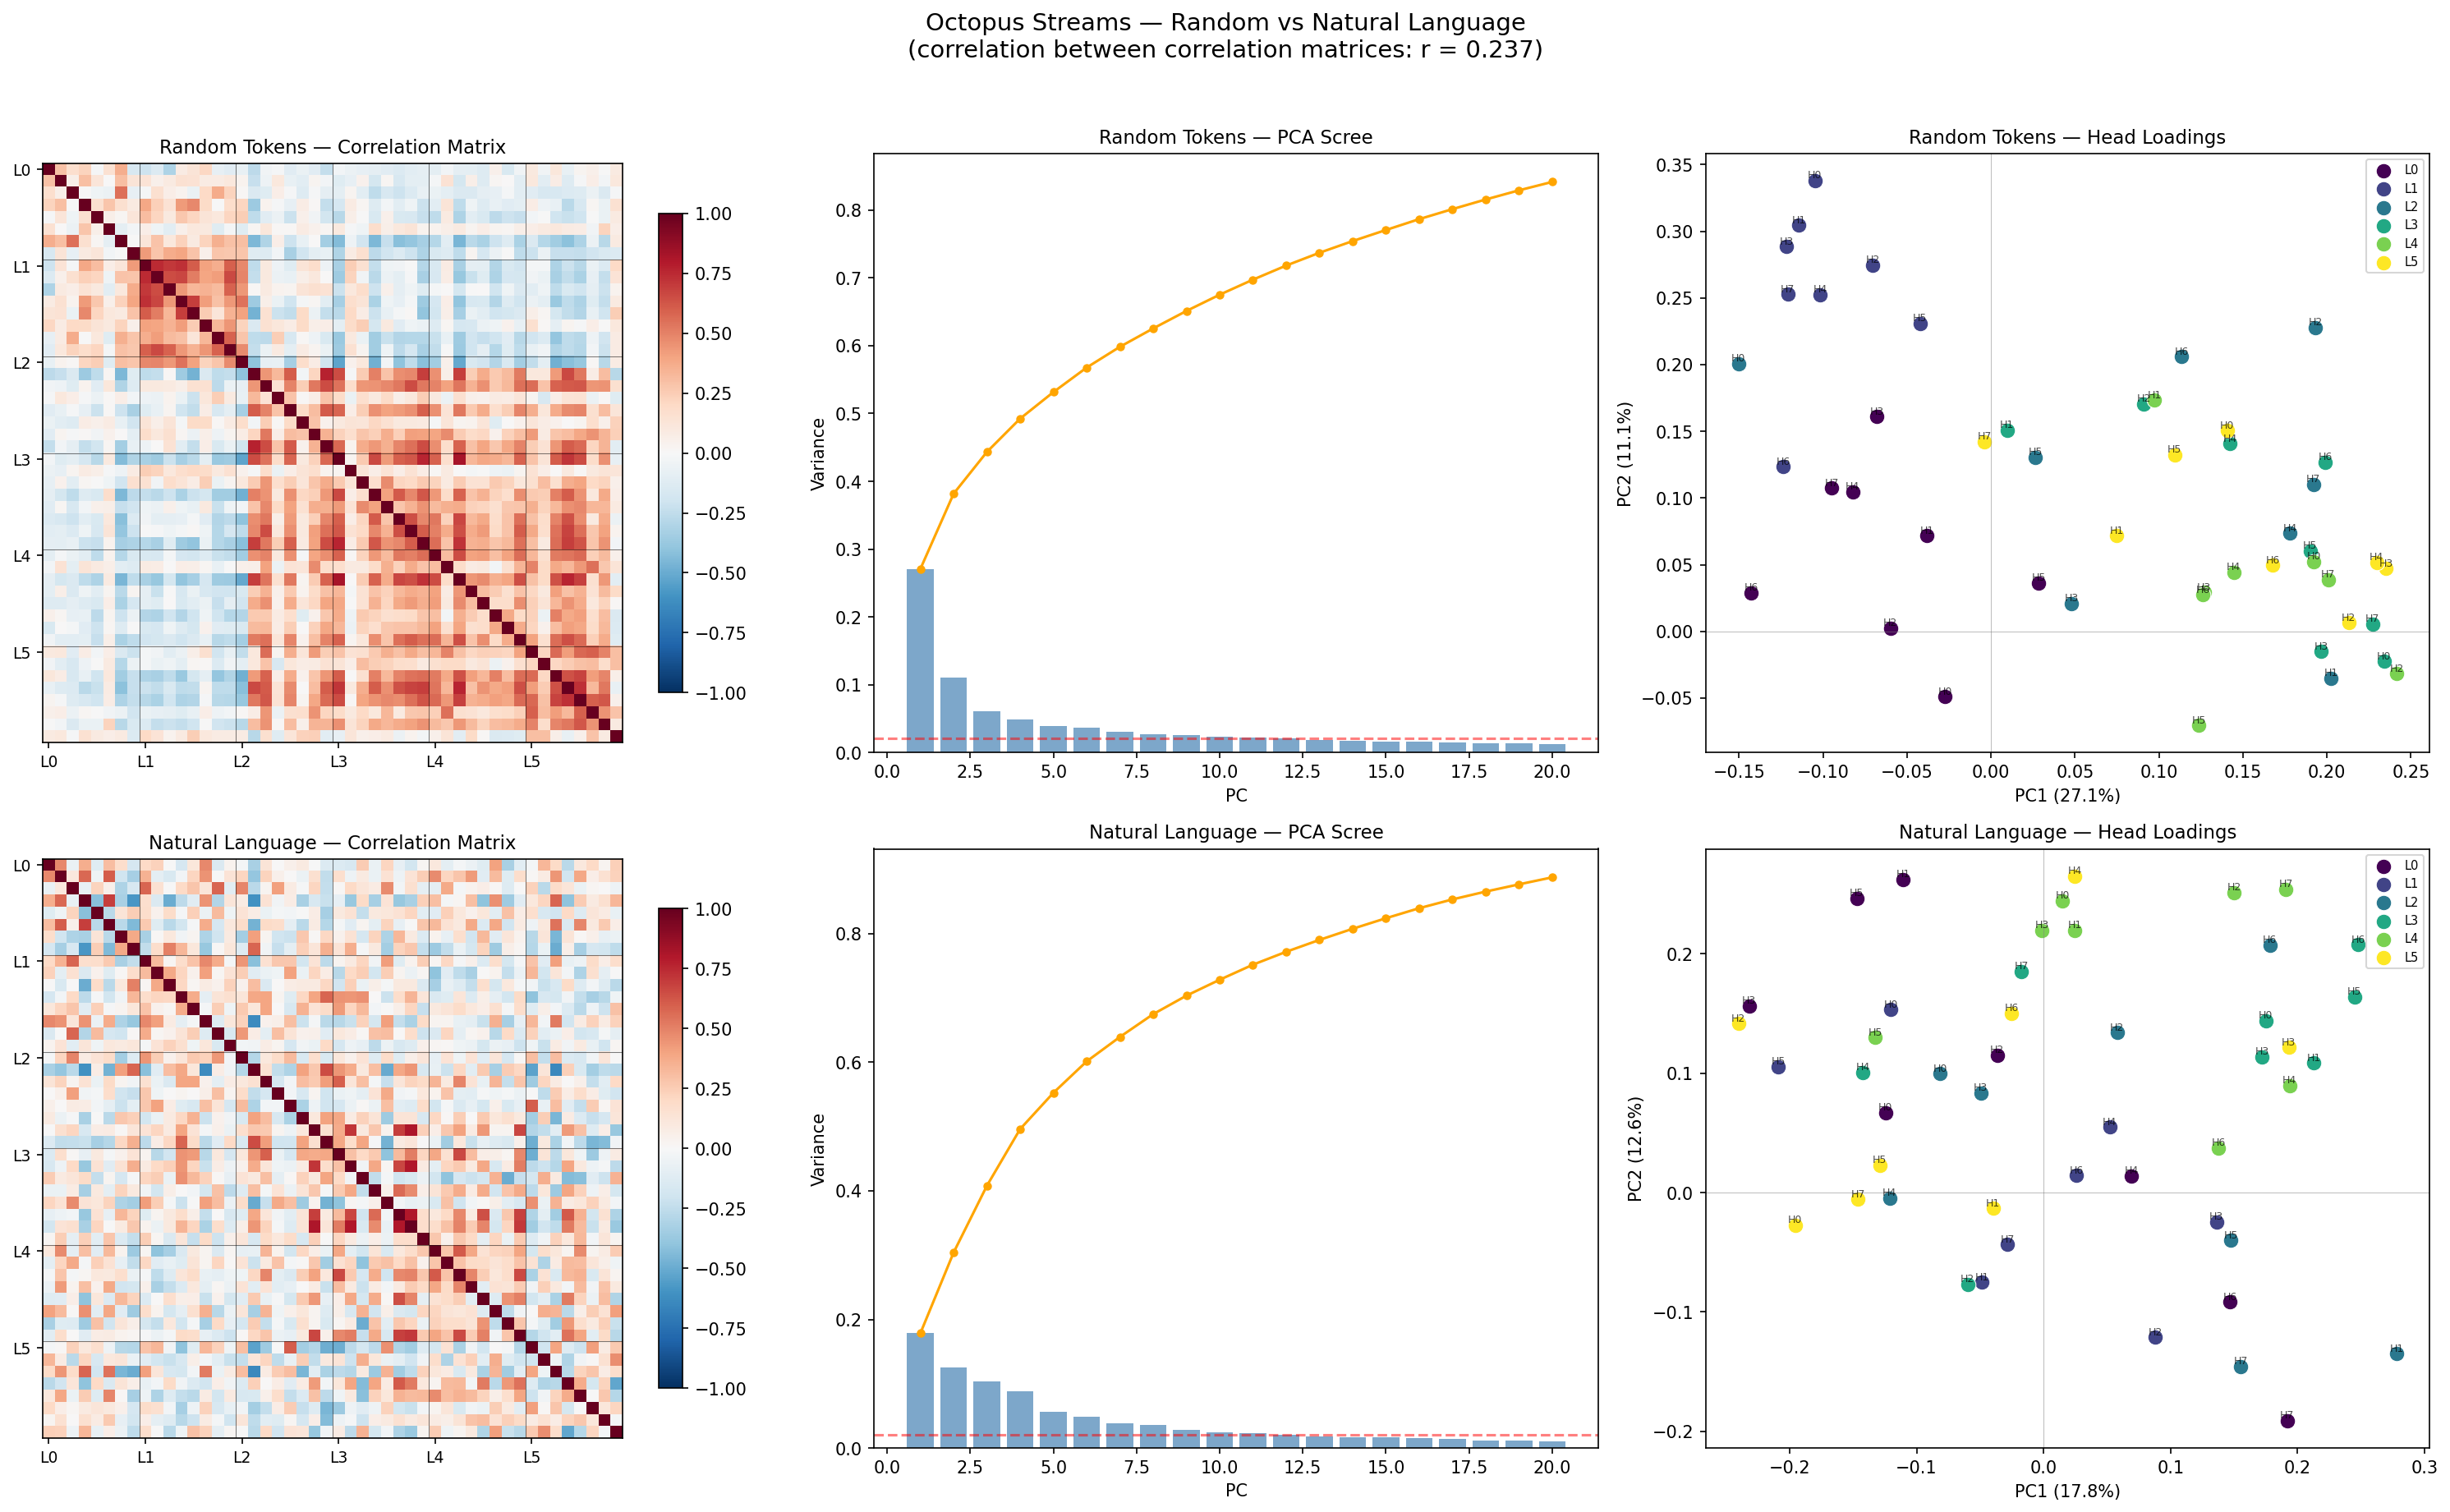
\includegraphics[width=\textwidth]{../results/04_comparison.png}
    \caption{Head-to-head correlation analysis. Top row: random token inputs. Bottom row: natural language (WikiText-103). Left: correlation matrices (red = positive, blue = negative). Centre: PCA scree plots. Right: head loadings on PC1 vs PC2, coloured by layer.}
    \label{fig:comparison}
\end{figure}

\paragraph{Random tokens.}
PC1 captures 27.1\% of variance.
The strongest correlations form a cross-layer chain: L3H0~$\leftrightarrow$~L4H2 ($r = 0.83$), L4H2~$\leftrightarrow$~L5H3 ($r = 0.76$).
The PCA biplot shows a clean separation: early-layer heads (L0, L1) load negatively on PC1, late-layer heads (L3, L4, L5) load positively.
Layer~2 is split.

\paragraph{Natural language.}
PC1 drops to 17.8\%, but the top 4 components are more evenly distributed (cumulative 49.6\% vs 49.2\%).
Components for 80\% variance: 14 (vs 17 for random), suggesting the structure is \emph{more concentrated} in the top PCs despite a weaker PC1.
The strongest correlations centre on \textbf{L3H6} as a hub: L2H6~$\leftrightarrow$~L3H6 ($r = 0.81$), L3H5~$\leftrightarrow$~L3H6 ($r = 0.80$), L3H1~$\leftrightarrow$~L3H6 ($r = 0.80$).

\paragraph{Cross-input comparison.}
The correlation between the two correlation matrices (upper triangle) is $r = 0.24$.
This indicates that the head co-activation structure \textbf{substantially reconfigures} depending on input type.
The model does not have fixed ``teams'' --- it has context-dependent coalitions.

%----------------------------------------------------------------------
\subsection{Ablation Results}
\label{sec:ablation-results}
%----------------------------------------------------------------------

Tables~\ref{tab:ablation-random} and \ref{tab:ablation-natural} show ablation results on constructed sentences and natural language respectively.

\begin{table}[h]
\centering
\begin{tabular}{lrrr}
\toprule
Ablation group & Heads & Perplexity & Ratio \\
\midrule
None (baseline) & 0 & 44.58 & 1.0$\times$ \\
Early arm (L0+L1) & 16 & 1{,}345.81 & 30.2$\times$ \\
Late arm (L3+L4+L5) & 24 & 1{,}051.64 & 23.6$\times$ \\
Layer~0 only & 8 & 952.23 & 21.4$\times$ \\
Layer~5 only & 8 & 60.08 & 1.3$\times$ \\
Correlated chain (L3H0+L4H2+L5H3) & 3 & 50.34 & 1.1$\times$ \\
Random 3 heads & 3 & 114.12 & 2.6$\times$ \\
\bottomrule
\end{tabular}
\caption{Ablation results on constructed sentences (random token inputs for correlation, short English sentences for ablation).}
\label{tab:ablation-random}
\end{table}

\begin{table}[h]
\centering
\begin{tabular}{lrrr}
\toprule
Ablation group & Heads & Perplexity & Ratio \\
\midrule
None (baseline) & 0 & 113.72 & 1.0$\times$ \\
Early arm (L0+L1) & 16 & 2{,}875.36 & 25.3$\times$ \\
Late arm (L3+L4+L5) & 24 & 1{,}909.57 & 16.8$\times$ \\
Layer~0 only & 8 & 2{,}019.60 & 17.8$\times$ \\
Layer~3 only & 8 & 510.41 & 4.5$\times$ \\
Layer~5 only & 8 & 146.06 & 1.3$\times$ \\
L3H6 cluster & 5 & 132.94 & 1.2$\times$ \\
Random-token chain (L3H0+L4H2+L5H3) & 3 & 122.93 & 1.1$\times$ \\
Random 5 heads (control) & 5 & 159.23 & 1.4$\times$ \\
\bottomrule
\end{tabular}
\caption{Ablation results on WikiText-103 natural language.}
\label{tab:ablation-natural}
\end{table}

\paragraph{Key findings.}

\begin{enumerate}[itemsep=4pt]

    \item \textbf{Layer~0 is catastrophically important.}
    Removing just 8 heads in Layer~0 causes 17.8--21.4$\times$ perplexity increase across both input types.
    Qualitatively, the model's output degenerates into formatting characters, pipe symbols, and fragments --- it loses basic language structure entirely.

    \item \textbf{Layer~5 is nearly dispensable.}
    Removing all 8 heads in Layer~5 causes only 1.3$\times$ damage on both input types.
    Output remains grammatical and contextually relevant, with only slight increases in repetition.

    \item \textbf{Early and late arms cause different kinds of damage.}
    Ablating the early arm (L0+L1) destroys \emph{syntax} --- the model can no longer form coherent token sequences.
    Ablating the late arm (L3+L4+L5) preserves syntax but destroys \emph{semantics} --- output is grammatical but vacuous (e.g., ``a group of three different kinds of data processing'').

    \item \textbf{Layer~3 is a middle-importance hub.}
    On natural language, Layer~3 ablation causes 4.5$\times$ damage --- intermediate between the extremes of L0 and L5.
    This is consistent with the correlation analysis identifying L3 as a coordination hub on natural-language inputs.

    \item \textbf{High correlation $\neq$ high importance.}
    The most strongly correlated head groups (the L3H0--L4H2--L5H3 chain on random tokens; the L3H6 cluster on natural language) cause \emph{less} damage when ablated than random head selections of the same size.
    Correlated heads appear to be \emph{redundant} --- their partners compensate when they are removed.

\end{enumerate}

%----------------------------------------------------------------------
\subsection{Domain Comparison}
\label{sec:domain-results}
%----------------------------------------------------------------------

Does the head coalition structure differ across linguistically distinct domains?
We repeat the correlation/PCA analysis from Experiments~1 and~4 on three additional domains: poetry, narrative prose, and Python code.
Figure~\ref{fig:domain-grid} shows the per-domain correlation matrices, scree plots, and PCA biplots.

\begin{figure}[h]
    \centering
    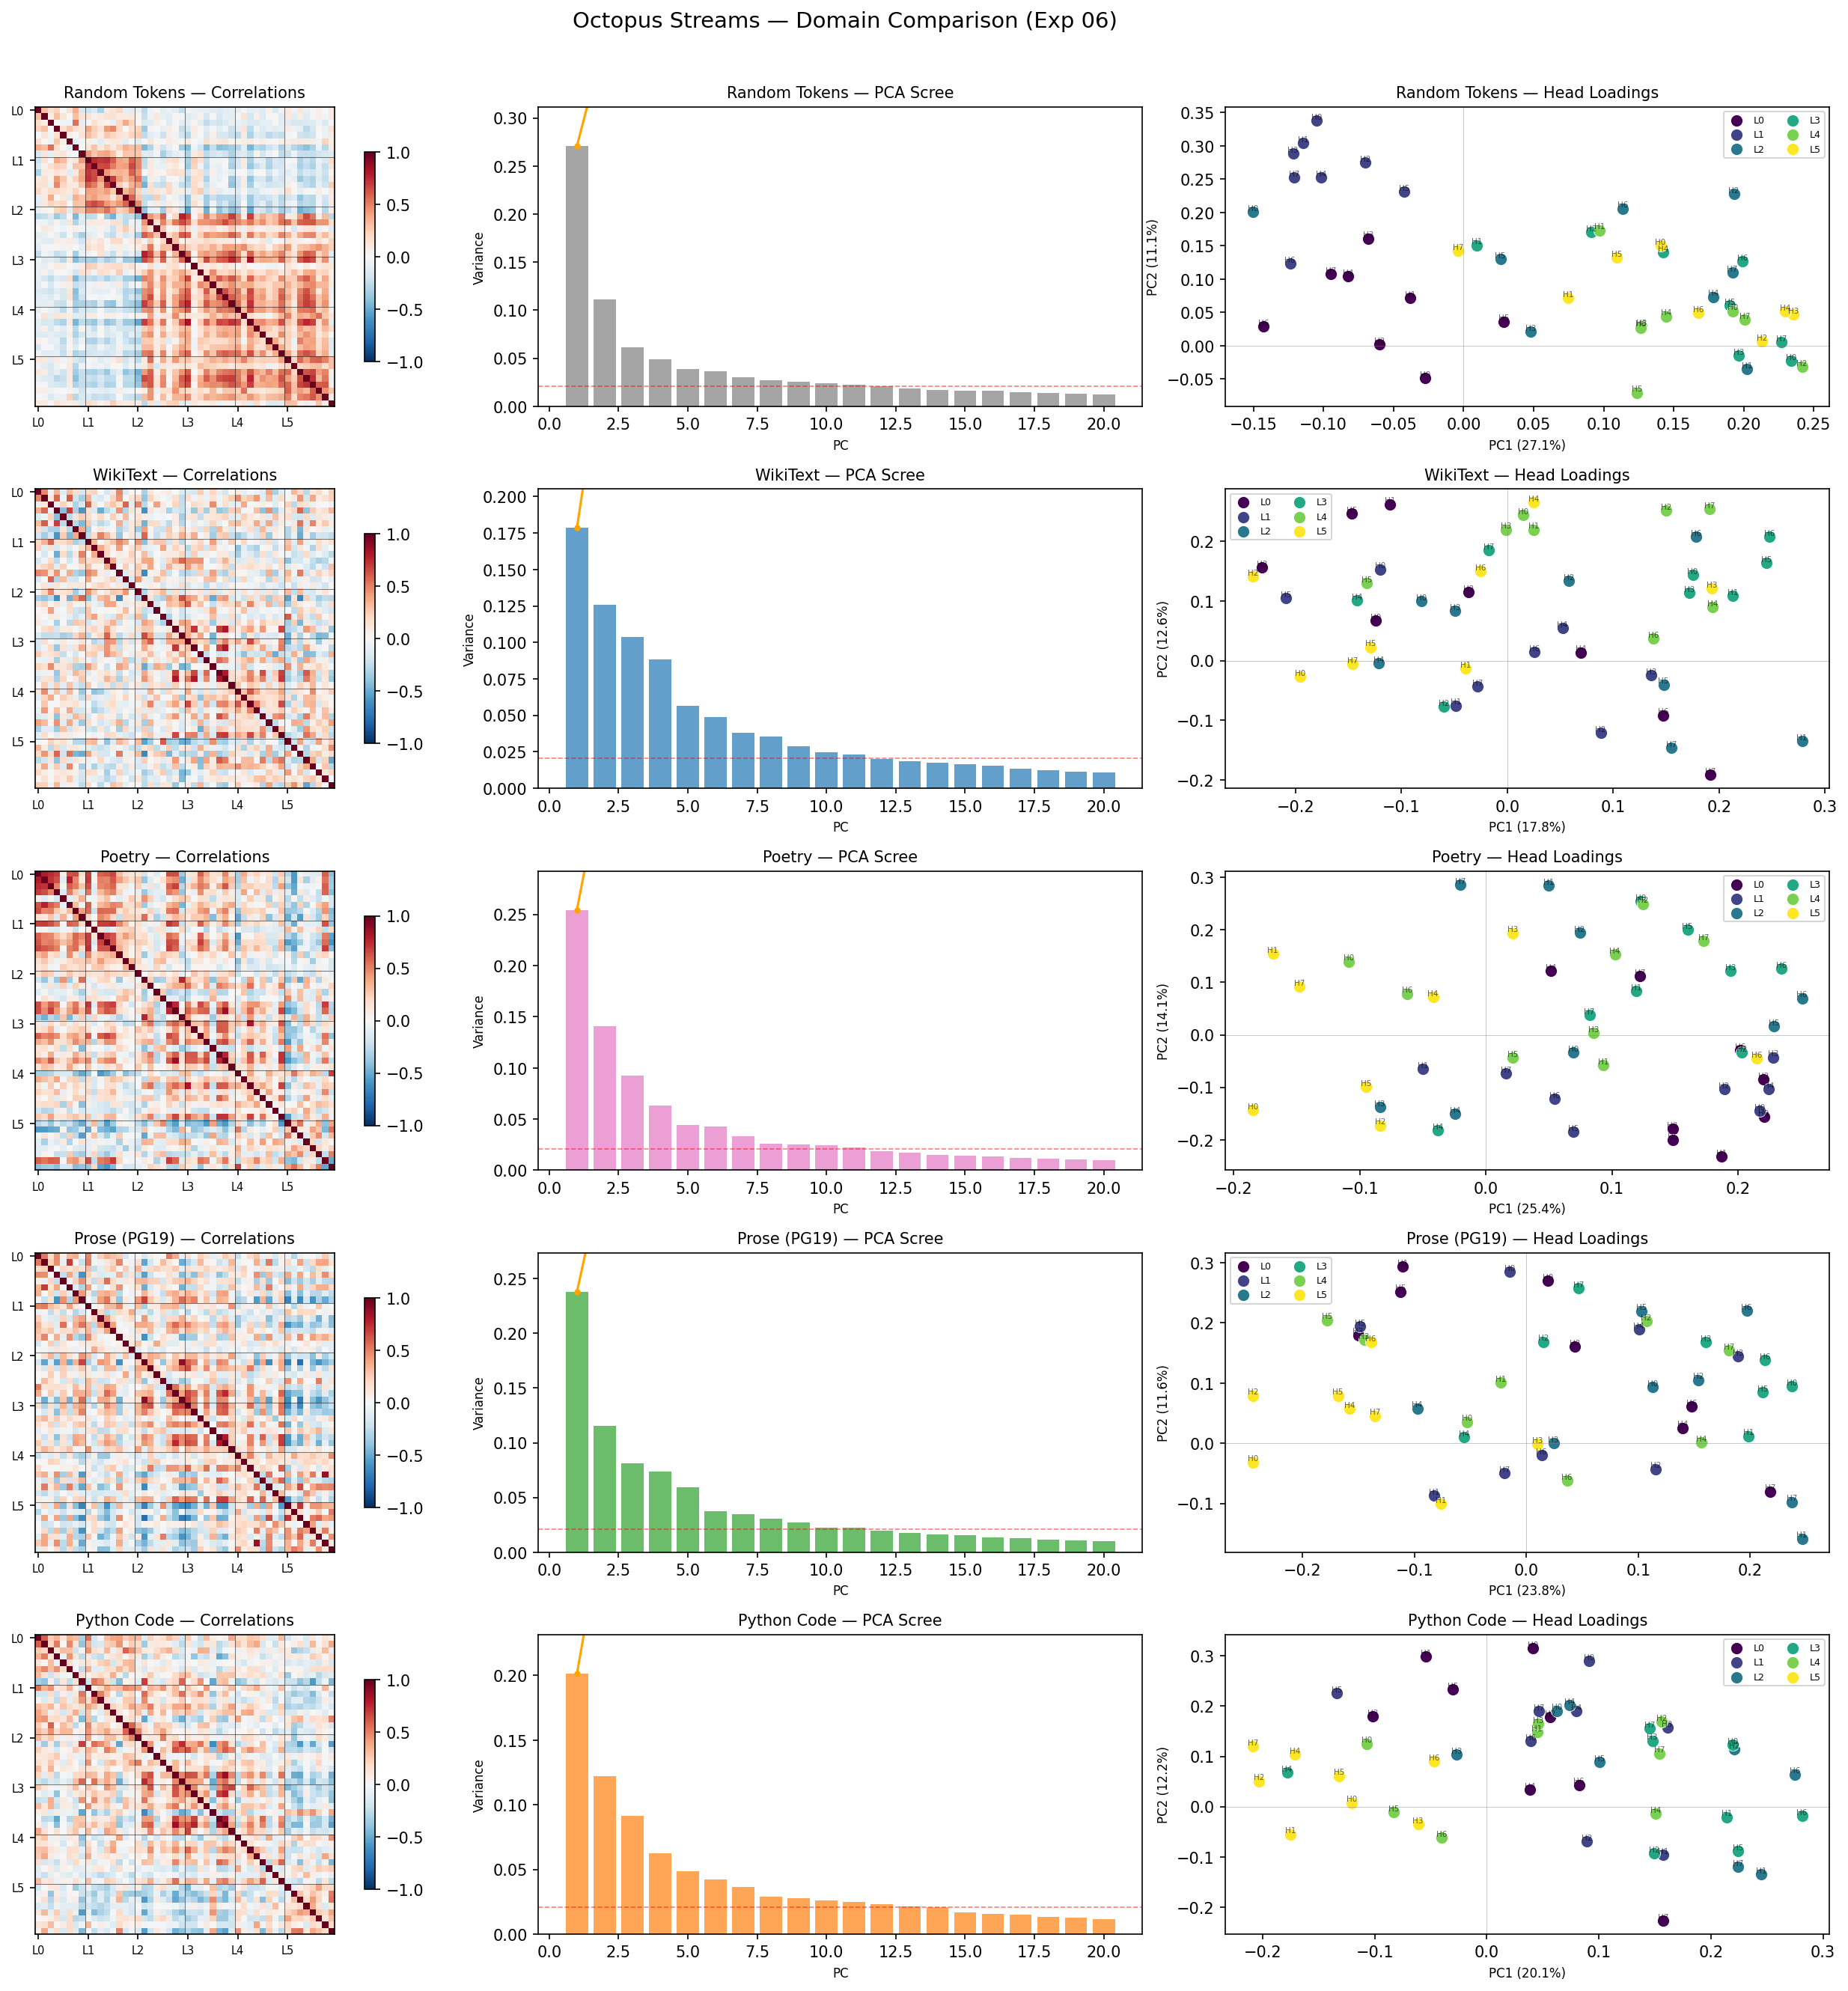
\includegraphics[width=\textwidth]{../results/06_domain_grid.png}
    \caption{Per-domain correlation analysis across all five input types. Each row shows one domain: correlation matrix (left), PCA scree plot (centre), and PC1/PC2 head loadings (right). Correlation matrices are ordered by layer; black lines mark layer boundaries.}
    \label{fig:domain-grid}
\end{figure}

\paragraph{Dimensionality varies by domain.}
Table~\ref{tab:domain-pca} summarises the PCA results.
Random tokens show the highest PC1 variance (27.1\%) but require the most components for 80\% total variance (17), while poetry shows the fewest (13).
This apparent paradox reflects different variance distributions: random inputs concentrate heavily on PC1 with a long tail, while natural-language domains spread variance more evenly across the top components.

\begin{table}[h]
\centering
\begin{tabular}{lrrr}
\toprule
Domain & PC1 & PC1+PC2 & Components for 80\% \\
\midrule
Random Tokens & 0.271 & 0.382 & 17 \\
WikiText & 0.178 & 0.304 & 14 \\
Poetry & 0.254 & 0.395 & 13 \\
Prose (Gutenberg) & 0.238 & 0.353 & 15 \\
Python Code & 0.201 & 0.323 & 16 \\
\bottomrule
\end{tabular}
\caption{PCA summary by domain. PC1 = fraction of variance explained by the first principal component. Components for 80\% = number of PCs needed to explain 80\% of total variance.}
\label{tab:domain-pca}
\end{table}

\paragraph{Natural-language domains form a shared coalition family.}
Figure~\ref{fig:similarity-matrix} shows the pairwise similarity between domains, measured as the Pearson correlation between the upper triangles of each pair's 48$\times$48 correlation matrices.

\begin{figure}[h]
    \centering
    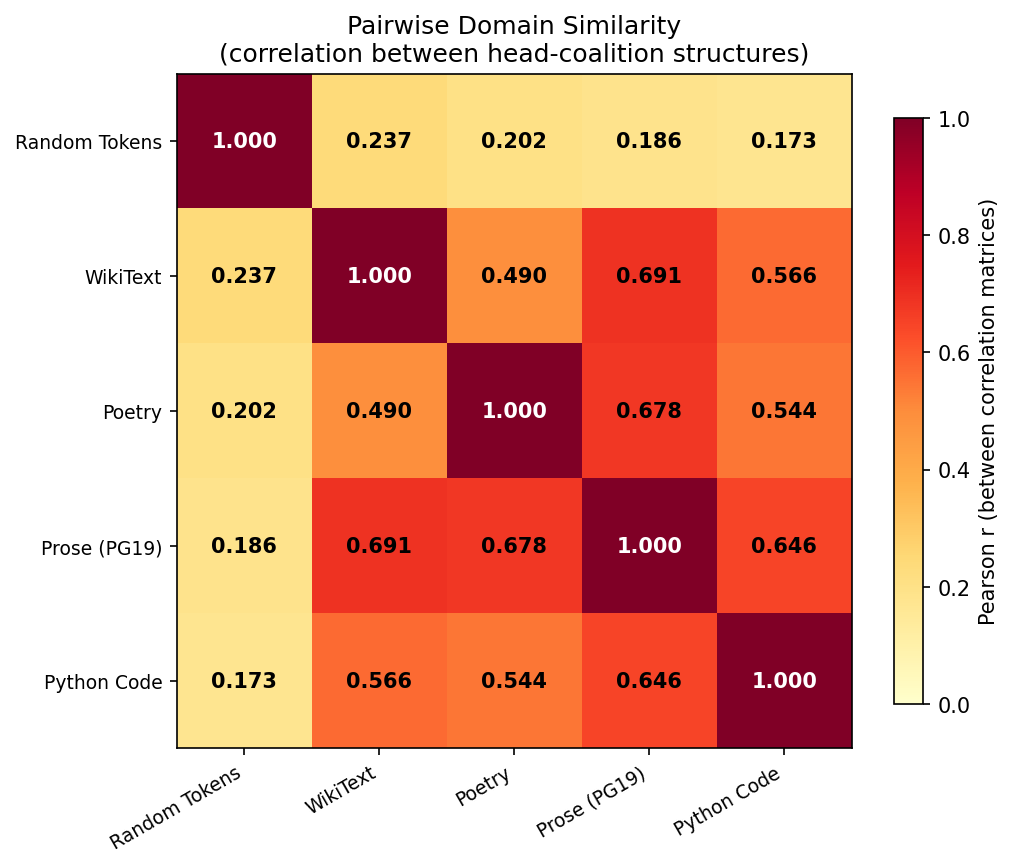
\includegraphics[width=0.65\textwidth]{../results/06_similarity_matrix.png}
    \caption{Pairwise domain similarity. Each cell shows the Pearson $r$ between two domains' head-to-head correlation matrices (upper triangle, 1{,}128 unique pairs). Darker = more similar coalition structure.}
    \label{fig:similarity-matrix}
\end{figure}

The results reveal a clear two-tier structure:

\begin{enumerate}[itemsep=4pt]
    \item \textbf{Random tokens are isolated.}
    Random-to-natural correlations range from $r = 0.17$ (code) to $r = 0.24$ (WikiText).
    This confirms and extends the Experiment~4 finding: the coalition structure under random inputs is fundamentally different from that under any form of real language.

    \item \textbf{Natural-language domains cluster together.}
    All pairwise correlations between real domains fall in the range $r = 0.49$--$0.69$.
    The strongest pair is WikiText~$\leftrightarrow$~Prose ($r = 0.691$), followed by Poetry~$\leftrightarrow$~Prose ($r = 0.678$).
    Despite large differences in vocabulary, style, and era (19th-century novels vs.\ 21st-century Wikipedia), these domains activate similar head coalitions.

    \item \textbf{Python code is the most alien real domain.}
    Code shows the lowest similarity to every other natural-language domain ($r = 0.54$--$0.65$), yet remains far closer to natural language than random tokens are.
    The model partially reconfigures for code but retains much of its natural-language coalition structure --- perhaps because Python inherits English keywords, naming conventions, and docstring prose.
\end{enumerate}

\paragraph{PCA overlay.}
Figure~\ref{fig:pca-overlay} plots the layer centroid trajectories for all five domains in the same PC space.
Each domain's PCA was computed independently, so axes are not directly comparable, but the \emph{shape} of each trajectory --- how the layer centroids trace through PC1--PC2 space --- reveals domain-specific patterns.
Random tokens show the widest excursion (especially Layer~0), while the four natural-language domains occupy a more compact region with similar trajectory shapes.

\begin{figure}[h]
    \centering
    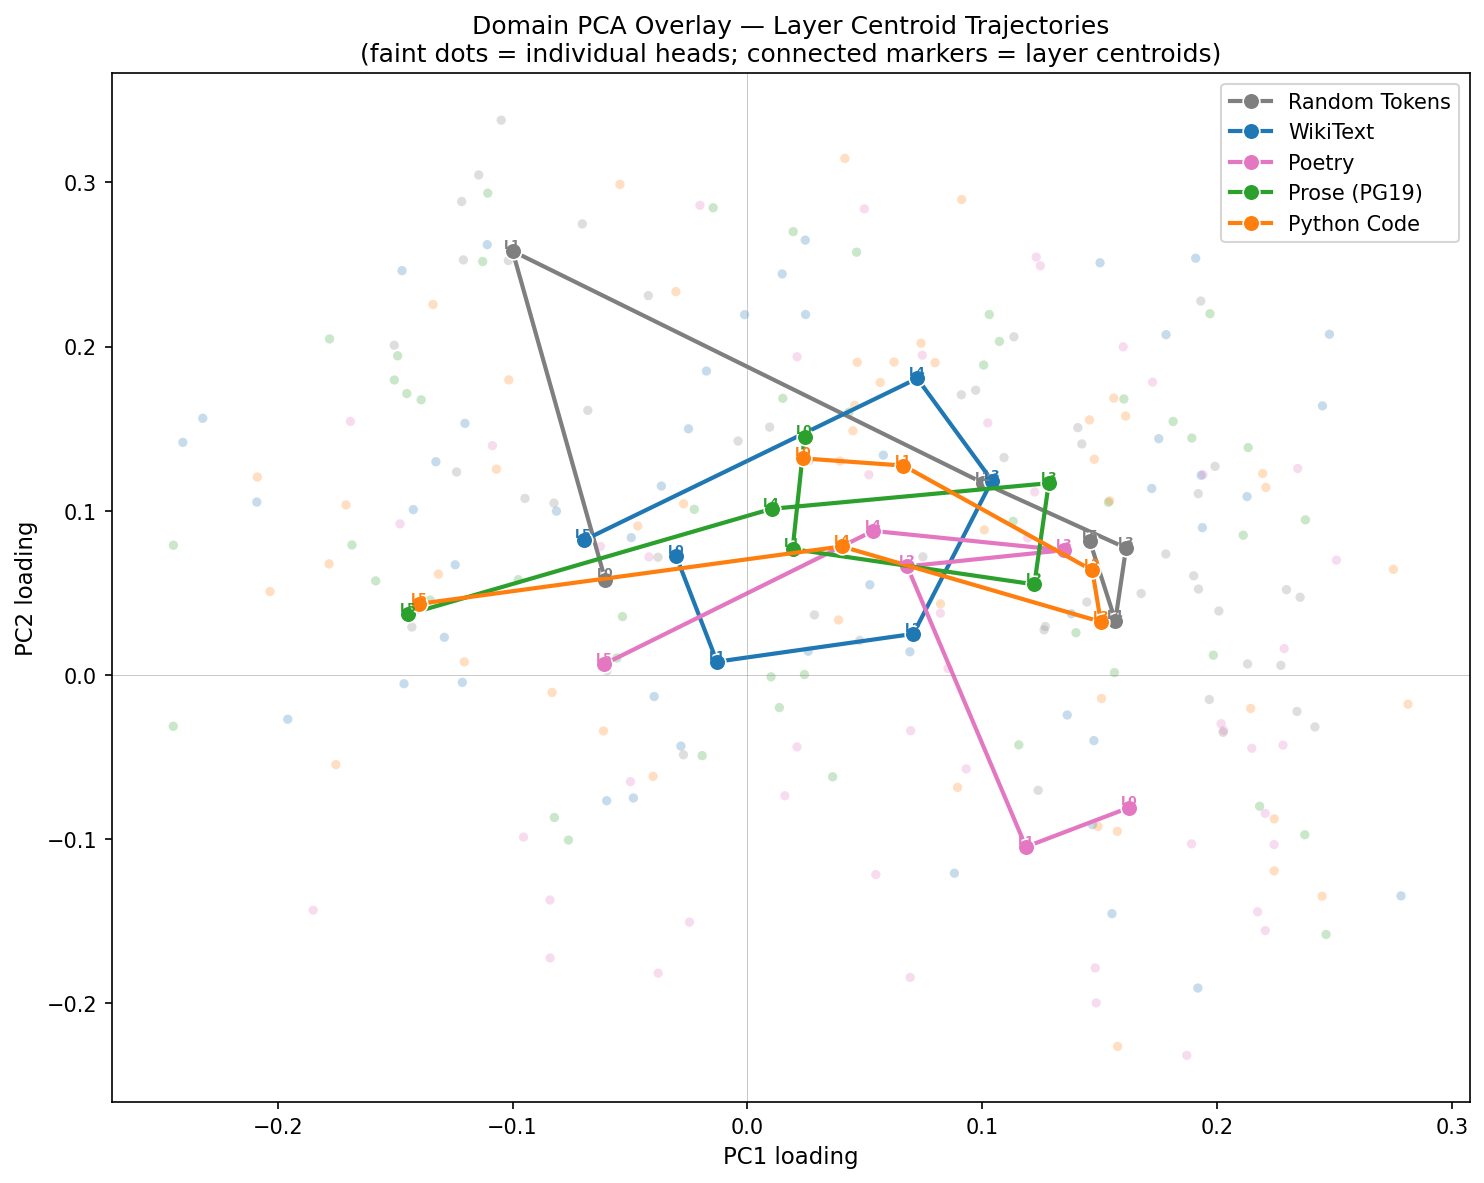
\includegraphics[width=0.75\textwidth]{../results/06_pca_overlay.png}
    \caption{PCA overlay showing layer centroid trajectories for all five domains. Faint dots are individual heads; connected markers trace the layer-by-layer centroid path for each domain. Each domain's PCA is computed independently.}
    \label{fig:pca-overlay}
\end{figure}

%----------------------------------------------------------------------
\subsection{Sparse Autoencoder Decomposition}
\label{sec:sae-results}
%----------------------------------------------------------------------

Experiments~1--6 operate at the level of whole attention heads: which heads co-activate, which are critical, and how coalitions shift across domains.
But each head writes a 64-dimensional vector into the 512-dimensional residual stream --- a representation that may encode many superimposed concepts (Section~\ref{sec:superposition}).
To look inside this representation, we train sparse autoencoders (SAEs) on the residual stream after Layers~0, 3, and~5.

\paragraph{Architecture.}
We use a \textbf{TopK} sparse autoencoder with $8\times$ expansion: the encoder projects the 512-dimensional residual stream into 4{,}096 features, of which exactly $k = 50$ are active per input (the top 50 pre-activations, passed through ReLU).
The decoder projects back to 512 dimensions; its columns are constrained to unit norm during training to prevent the encoder from collapsing features into the decoder bias.

We chose the TopK architecture over the more common ReLU+L1 approach after extensive experimentation.
ReLU+L1 SAEs control sparsity through an L1 penalty on the hidden activations, but we found this fundamentally unable to achieve the target sparsity: even with aggressive L1 coefficients ($\lambda$ up to $0.128$, a $256\times$ increase from the starting value), the L0 norm remained stuck near 1{,}400 active features per input --- far above our target of 20--100.
The failure mode is that many features hover at small positive activations, each contributing too little to reconstruction for the L1 gradient to kill them, but collectively accounting for most of the representation.
TopK eliminates this problem by construction: exactly $k$ features are active, always.

\paragraph{Training.}
Each SAE was trained for 50{,}000 steps on residual-stream activations from 2{,}000 WikiText-103 sequences (256k positions), with Adam (lr = $3 \times 10^{-4}$) and MSE reconstruction loss.
Activations were normalised to unit variance before training, with the scale factor stored per layer for use during inference.
Training took approximately 30 minutes total for all three layers on Apple MPS.

\paragraph{Feature census.}
We classify each of the 4{,}096 features by how many of the five domains (random, WikiText, poetry, prose, code) activate it above a threshold of $10^{-3}$.
Table~\ref{tab:feature-census} shows the results.

\begin{table}[h]
\centering
\begin{tabular}{lrrrrr}
\toprule
Layer & Alive & Dead (\%) & Universal & Shared & Domain-specific \\
\midrule
0 & 3{,}781 & 315 (7.7\%) & 3{,}504 (92.7\%) & 248 (6.6\%) & 29 (0.8\%) \\
3 & 3{,}673 & 423 (10.3\%) & 1{,}629 (44.4\%) & 1{,}776 (48.4\%) & 268 (7.3\%) \\
5 & 438 & 3{,}658 (89.3\%) & 329 (75.1\%) & 77 (17.6\%) & 32 (7.3\%) \\
\bottomrule
\end{tabular}
\caption{Feature census by layer. Universal = active in all 5 domains; Shared = active in 2--4 domains; Domain-specific = active in exactly 1 domain. Percentages are of alive features. Layer~5's 89.3\% dead rate reflects that the final layer concentrates its representation into far fewer features.}
\label{tab:feature-census}
\end{table}

\paragraph{Layer~0: universal infrastructure.}
92.7\% of Layer~0's alive features are universal --- active across all five domains, including random tokens.
These features respond to basic token-level properties: punctuation detectors (comma, period, closing parenthesis), common function words (``the'', ``a'', ``of'', ``in''), and the end-of-text token.
Only 29 features (0.8\%) are domain-specific.
This matches the ablation finding that Layer~0 is catastrophically important (17.8$\times$ perplexity): it builds domain-agnostic representations that every subsequent layer depends on.

\paragraph{Layer~3: the reconfiguration hub.}
Layer~3 shows a dramatically different profile: only 44.4\% of features are universal, while 48.4\% are shared (active in 2--4 domains) and 7.3\% are domain-specific.
This is the layer with the largest pool of features that \emph{change behaviour} depending on the input domain --- exactly what we would expect of a coordination hub that reconfigures for different text types (Section~\ref{sec:domain-results}).
Its top features include period/sentence-boundary detectors, capital-letter features, and features that respond differently to code vs.\ prose.

\paragraph{Layer~5: concentrated output.}
Layer~5 has 89.3\% dead features, with only 438 of 4{,}096 alive.
This extreme sparsity suggests that the final layer has converged to a small set of output-relevant features --- consistent with its near-dispensability in ablation (1.3$\times$ perplexity).
Among its alive features, several are currency/number detectors (``\pounds'', ``\$'') and quotation-mark features, consistent with specialisation for next-token prediction of specific token classes.

\paragraph{Limitations.}
These results should be interpreted cautiously.
The TopK architecture \emph{forces} exactly 50 features to be active per input, which imposes structure that may not reflect the true sparsity of the underlying representation.
The domain classification depends on an arbitrary activation threshold ($10^{-3}$).
Most importantly, the max-activating tokens for each feature provide post-hoc labels, not causal evidence --- we have not verified that these features are causally involved in the computations we attribute to them.
The feature census reveals the \emph{shape} of each layer's representation (how many features are shared vs.\ specialised) more reliably than it identifies \emph{what} any individual feature computes.

\begin{figure}[h]
    \centering
    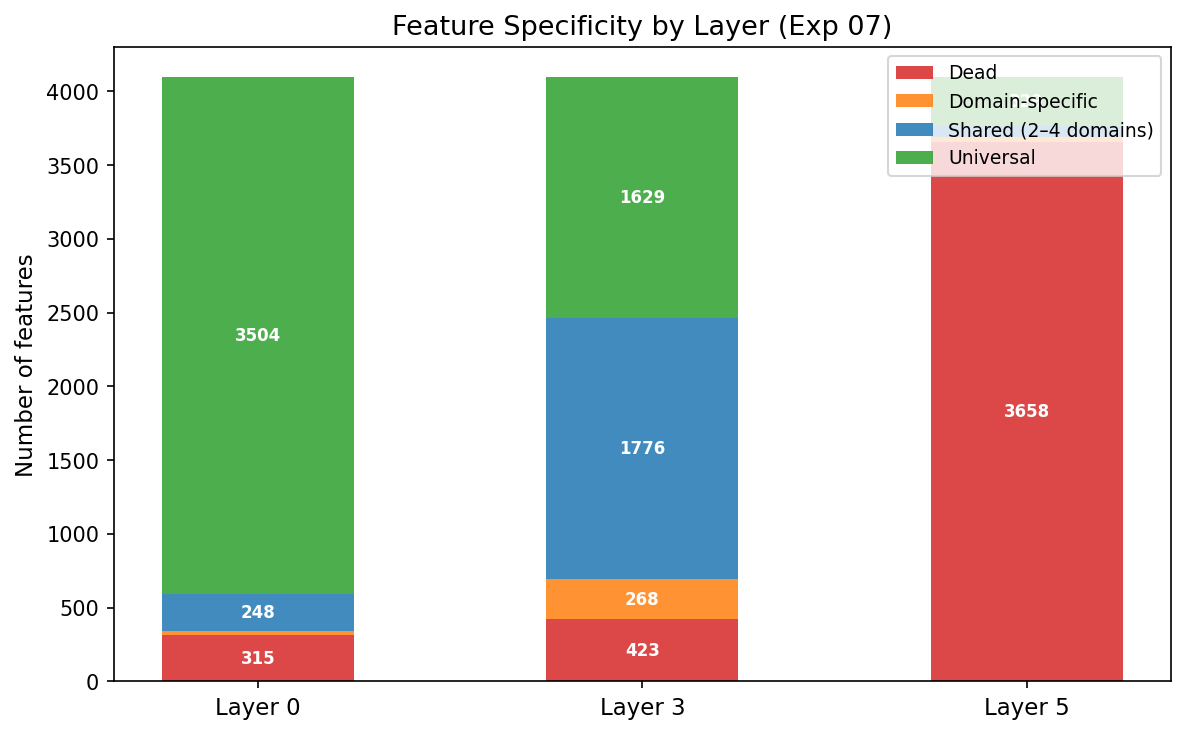
\includegraphics[width=\textwidth]{../results/07_feature_specificity.png}
    \caption{Feature specificity by layer. Each bar shows the fraction of 4{,}096 features that are dead, universal (active in all 5 domains), shared (2--4 domains), or domain-specific (1 domain). Layer~0 is almost entirely universal; Layer~3 has the most domain-sensitive features; Layer~5 is mostly dead.}
    \label{fig:feature-specificity}
\end{figure}

%----------------------------------------------------------------------
\subsection{Direct Head Interpretation}
\label{sec:head-interp}
%----------------------------------------------------------------------

Experiments~1--7 treat attention heads as black boxes, measuring their output norms and correlations without asking \emph{what} each head computes.
To bridge this gap, we directly examine the 8~heads in Layer~3 --- the coordination hub identified by correlation analysis (Section~\ref{sec:corr-results}), ablation (4.5$\times$ perplexity damage, Section~\ref{sec:ablation-results}), and SAE decomposition (most domain-sensitive feature repertoire, Section~\ref{sec:sae-results}).

For each head we measure three things:
\begin{enumerate}[itemsep=2pt]
    \item \textbf{Attention pattern}: where does the head look? We classify heads by their dominant attention target: the beginning-of-sequence (BOS) token, the previous token, or a broad distribution across the context window.
    \item \textbf{Direct logit attribution (DLA)}: what does the head's output mean? We project each head's mean output vector through the unembedding matrix $W_U$ to identify which tokens it promotes or suppresses in the next-token prediction.
    \item \textbf{Domain sensitivity}: how much does the head's output magnitude vary across our five domains?
\end{enumerate}

\paragraph{Most heads attend to BOS.}
Table~\ref{tab:head-types} and Figure~\ref{fig:attention-patterns} summarise the results.
Five of the eight heads (H0, H1, H3, H5, H6) primarily attend to the beginning-of-sequence token, with BOS attention ranging from 40\% (H3) to 87\% (H1).
Only two heads (H2 and H7) distribute attention broadly across the context, and one (H4) attends primarily to the previous token and itself.

\begin{table}[h]
\centering
\small
\begin{tabular}{llrrrl}
\toprule
Head & Type & BOS\% & Entropy & Domain ratio & Notable logit signal \\
\midrule
L3H0 & BOS & 62.8 & 0.48 & 1.3$\times$ & Promotes punctuation \\
L3H1 & BOS & 87.1 & 0.20 & 1.2$\times$ & Promotes content words, suppresses markup \\
L3H2 & Distributed & 8.7 & 0.89 & 1.4$\times$ & Promotes ellipsis, \textbf{suppresses whitespace ($-$5.7)} \\
L3H3 & BOS & 40.1 & 0.76 & 1.3$\times$ & Promotes sports/competition terms \\
L3H4 & Local & 8.8 & 0.60 & \textbf{1.7$\times$} & Suppresses Unicode garbage ($-$3.6) \\
L3H5 & BOS & 70.3 & 0.41 & 1.1$\times$ & Near-dormant (norms $\approx$ 1.0) \\
L3H6 & BOS & 72.9 & 0.37 & 1.4$\times$ & Code-sensitive; suppresses programming tokens \\
L3H7 & Distributed & 29.5 & 0.72 & 1.5$\times$ & Broad content terms \\
\bottomrule
\end{tabular}
\caption{Layer~3 head characterisation. BOS\% = fraction of attention directed to the beginning-of-sequence token. Entropy = normalised attention entropy (0 = focused, 1 = uniform). Domain ratio = ratio of maximum to minimum output norm across five domains. Logit signals from direct logit attribution on WikiText inputs.}
\label{tab:head-types}
\end{table}

\begin{figure}[h]
    \centering
    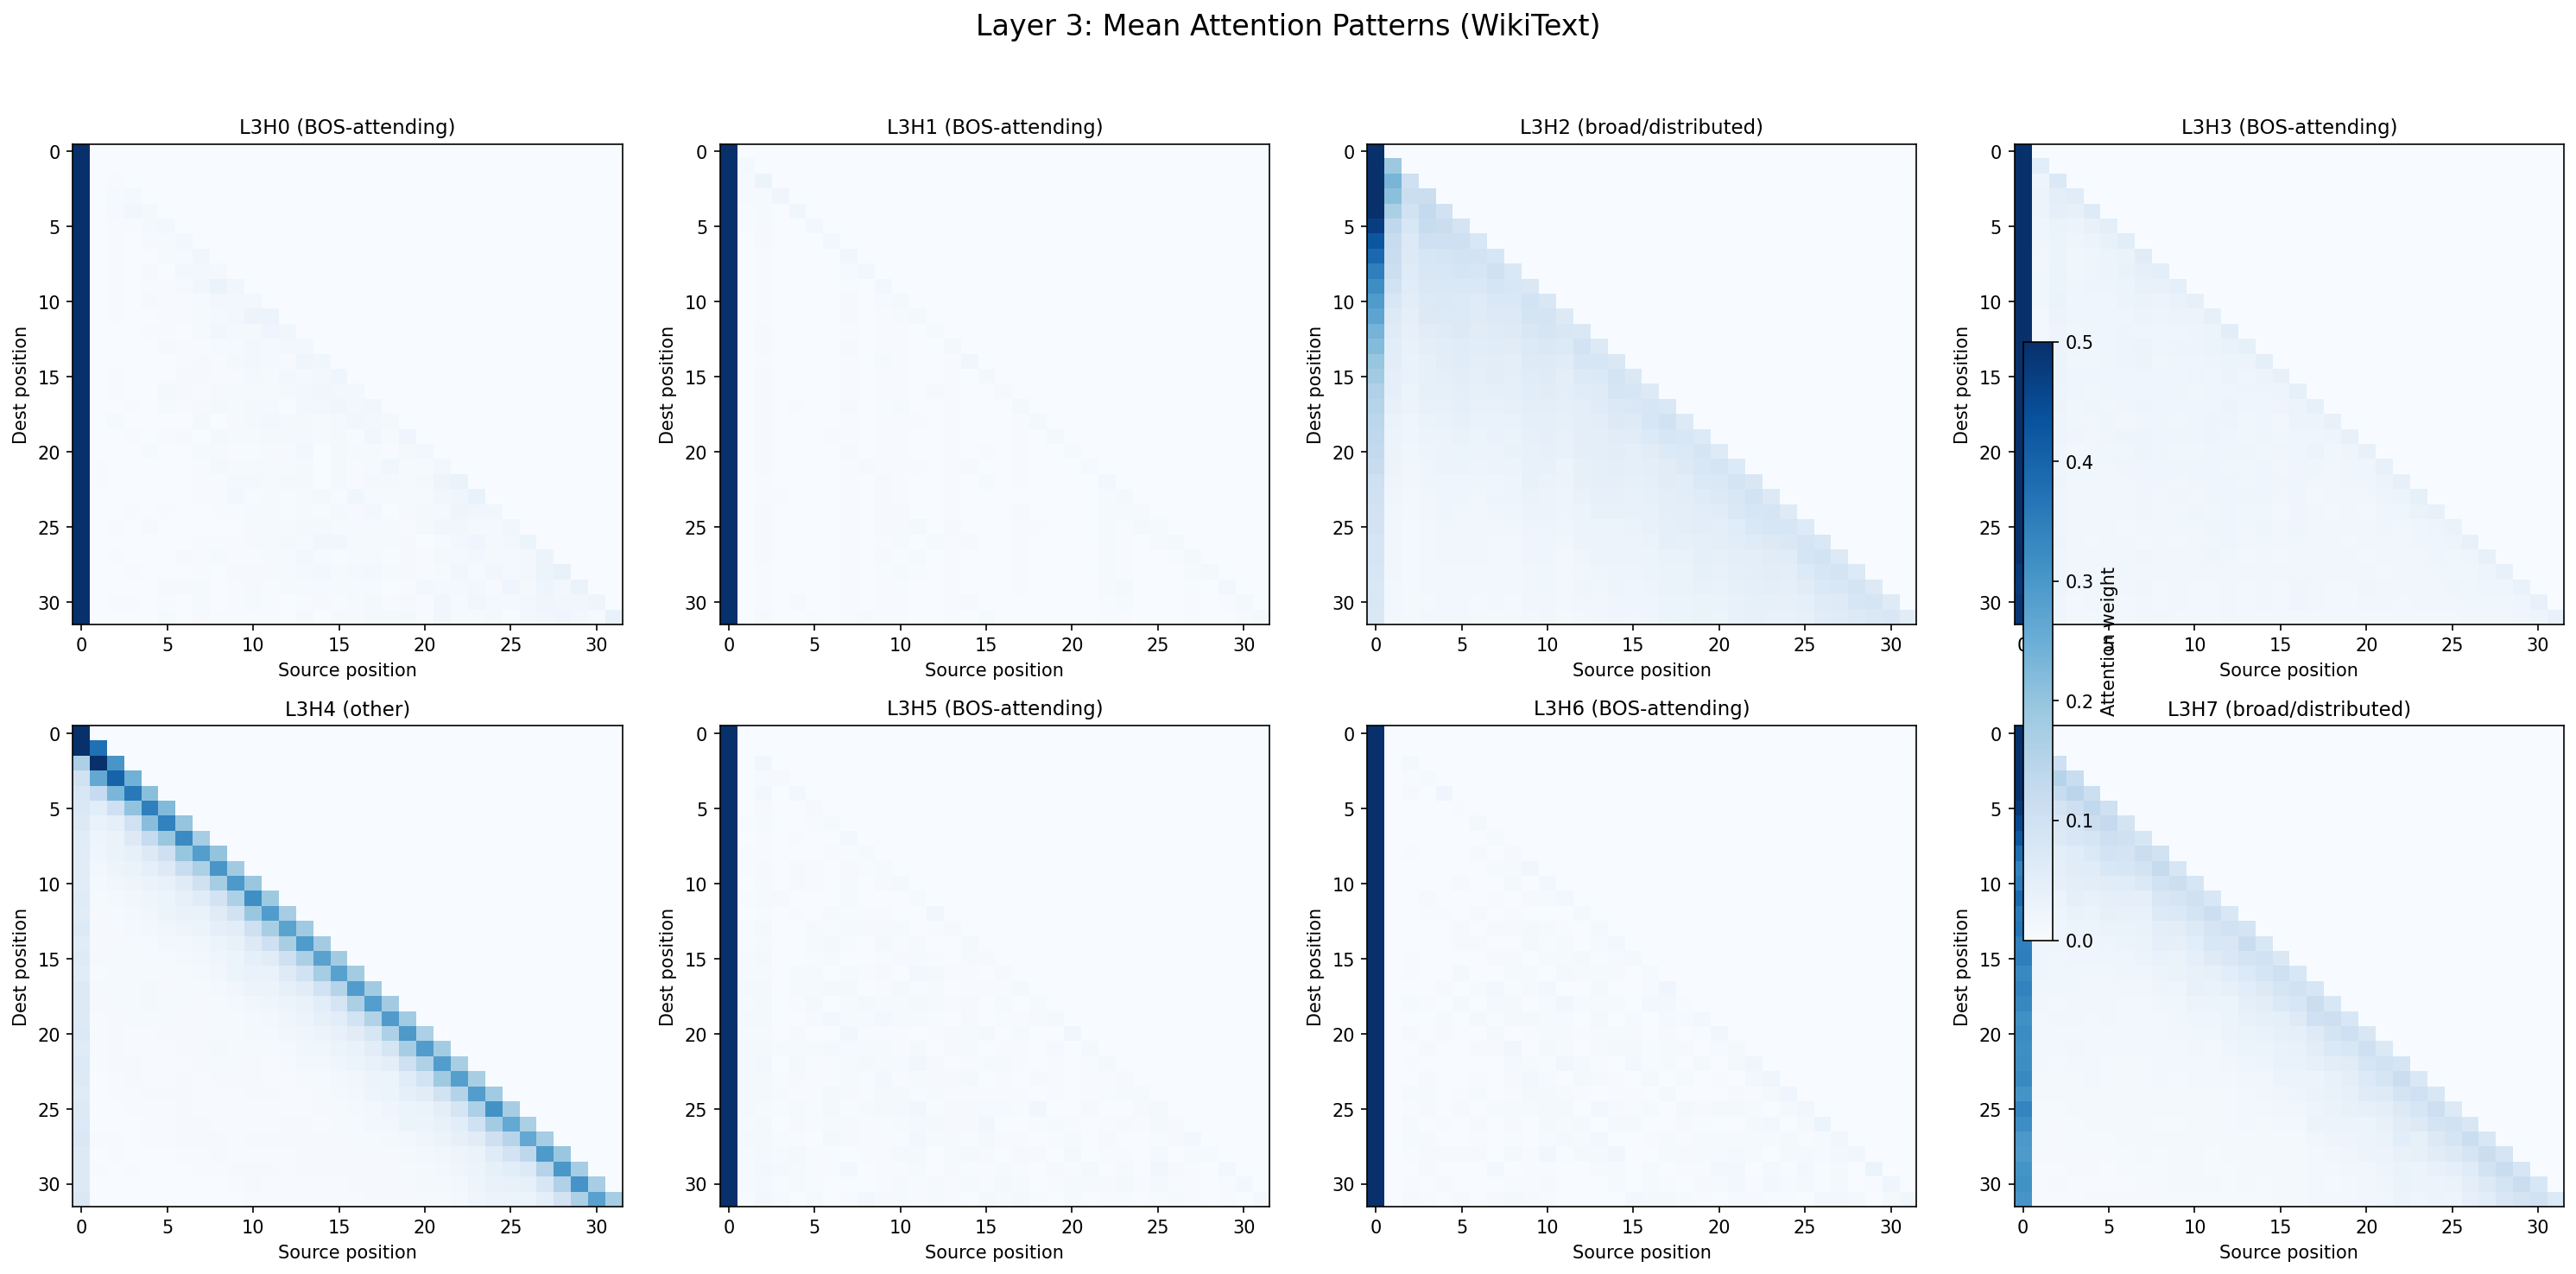
\includegraphics[width=\textwidth]{../results/08_L3_attention_patterns.png}
    \caption{Mean attention patterns for each Layer~3 head on WikiText (first 32 positions). A bright leftmost column indicates BOS attention. Five heads (H0, H1, H3, H5, H6) attend primarily to BOS. H2 shows diffuse contextual attention; H4 shows a strong diagonal (previous-token and self-attention).}
    \label{fig:attention-patterns}
\end{figure}

The prevalence of BOS-attending heads is striking but consistent with the mechanistic interpretability literature, where BOS attention is understood as a ``parking'' mechanism --- when a head has no contextually useful query, it directs attention to BOS as a neutral default.
But the logit attribution reveals that these BOS-attending heads are not idle: they contribute substantial biases to the next-token prediction.
L3H1, despite attending almost exclusively to BOS (87\%), writes the largest output vectors in the layer (norms 2.4--2.7) and promotes common English content words (``satisfied,'' ``depending,'' ``families,'' ``them'') while suppressing markup tokens (``\texttt{======},'' ``\texttt{-{}-{}->},'' ``\texttt{\textasciitilde\textasciitilde\textasciitilde}'').
It functions as a \emph{content-word prior}: a constant bias toward natural language and away from formatting.

\paragraph{Two heads do the contextual work.}
Heads H2 and H4 stand out as the only heads that attend meaningfully to the input context rather than BOS.

\textbf{H2} (broad/distributed, entropy = 0.89) exhibits an exceptionally strong whitespace-suppression function.
Its top suppressed tokens are all whitespace variants, with logit contributions of $-5.67$ --- by far the strongest single-head signal in the layer.
Simultaneously, it promotes ellipsis and continuation tokens ($+3.2$).
This head appears to function as a \emph{continuation enforcer}: it pushes the model away from generating empty space and toward continuing the text.
Its domain sensitivity (1.4$\times$, strongest for code) is consistent with this role, since code contains more structured whitespace that needs careful management.

\textbf{H4} (local-context, entropy = 0.60) attends primarily to the previous token (29\%) and itself (19\%), with the shortest average lookback in the layer (8.4 tokens) and highest domain sensitivity (\textbf{1.7$\times$}).
It strongly suppresses Unicode replacement characters (logit $-3.6$), functioning as a \emph{garbage filter}.
Its output norms nearly double between random tokens (1.33) and WikiText (2.29), confirming that it activates selectively for structured input --- the largest domain gap of any head in the layer (Figure~\ref{fig:head-profiles}).

\paragraph{The hub head is a bias signal.}
One of the most notable findings is that L3H6 --- identified in Section~\ref{sec:corr-results} as the central hub of the natural-language correlation structure ($r = 0.80$--$0.81$ with three other heads) --- is a BOS-attending head with low output norms (0.92--1.31).
It contributes primarily by suppressing programming-related tokens and shows its highest output norm on code (1.31 vs.\ 0.92 for random).
Its hub status in the correlation analysis arises not from performing contextually complex computation but from providing a \emph{domain-sensitive bias signal} that co-varies with other heads: when the input is code, it writes a larger output that co-activates with other code-responsive heads.
This reframes the meaning of ``hub'' in our correlation structure --- it need not be a computational linchpin but rather a shared reference signal that indexes the input domain.

\begin{figure}[h]
    \centering
    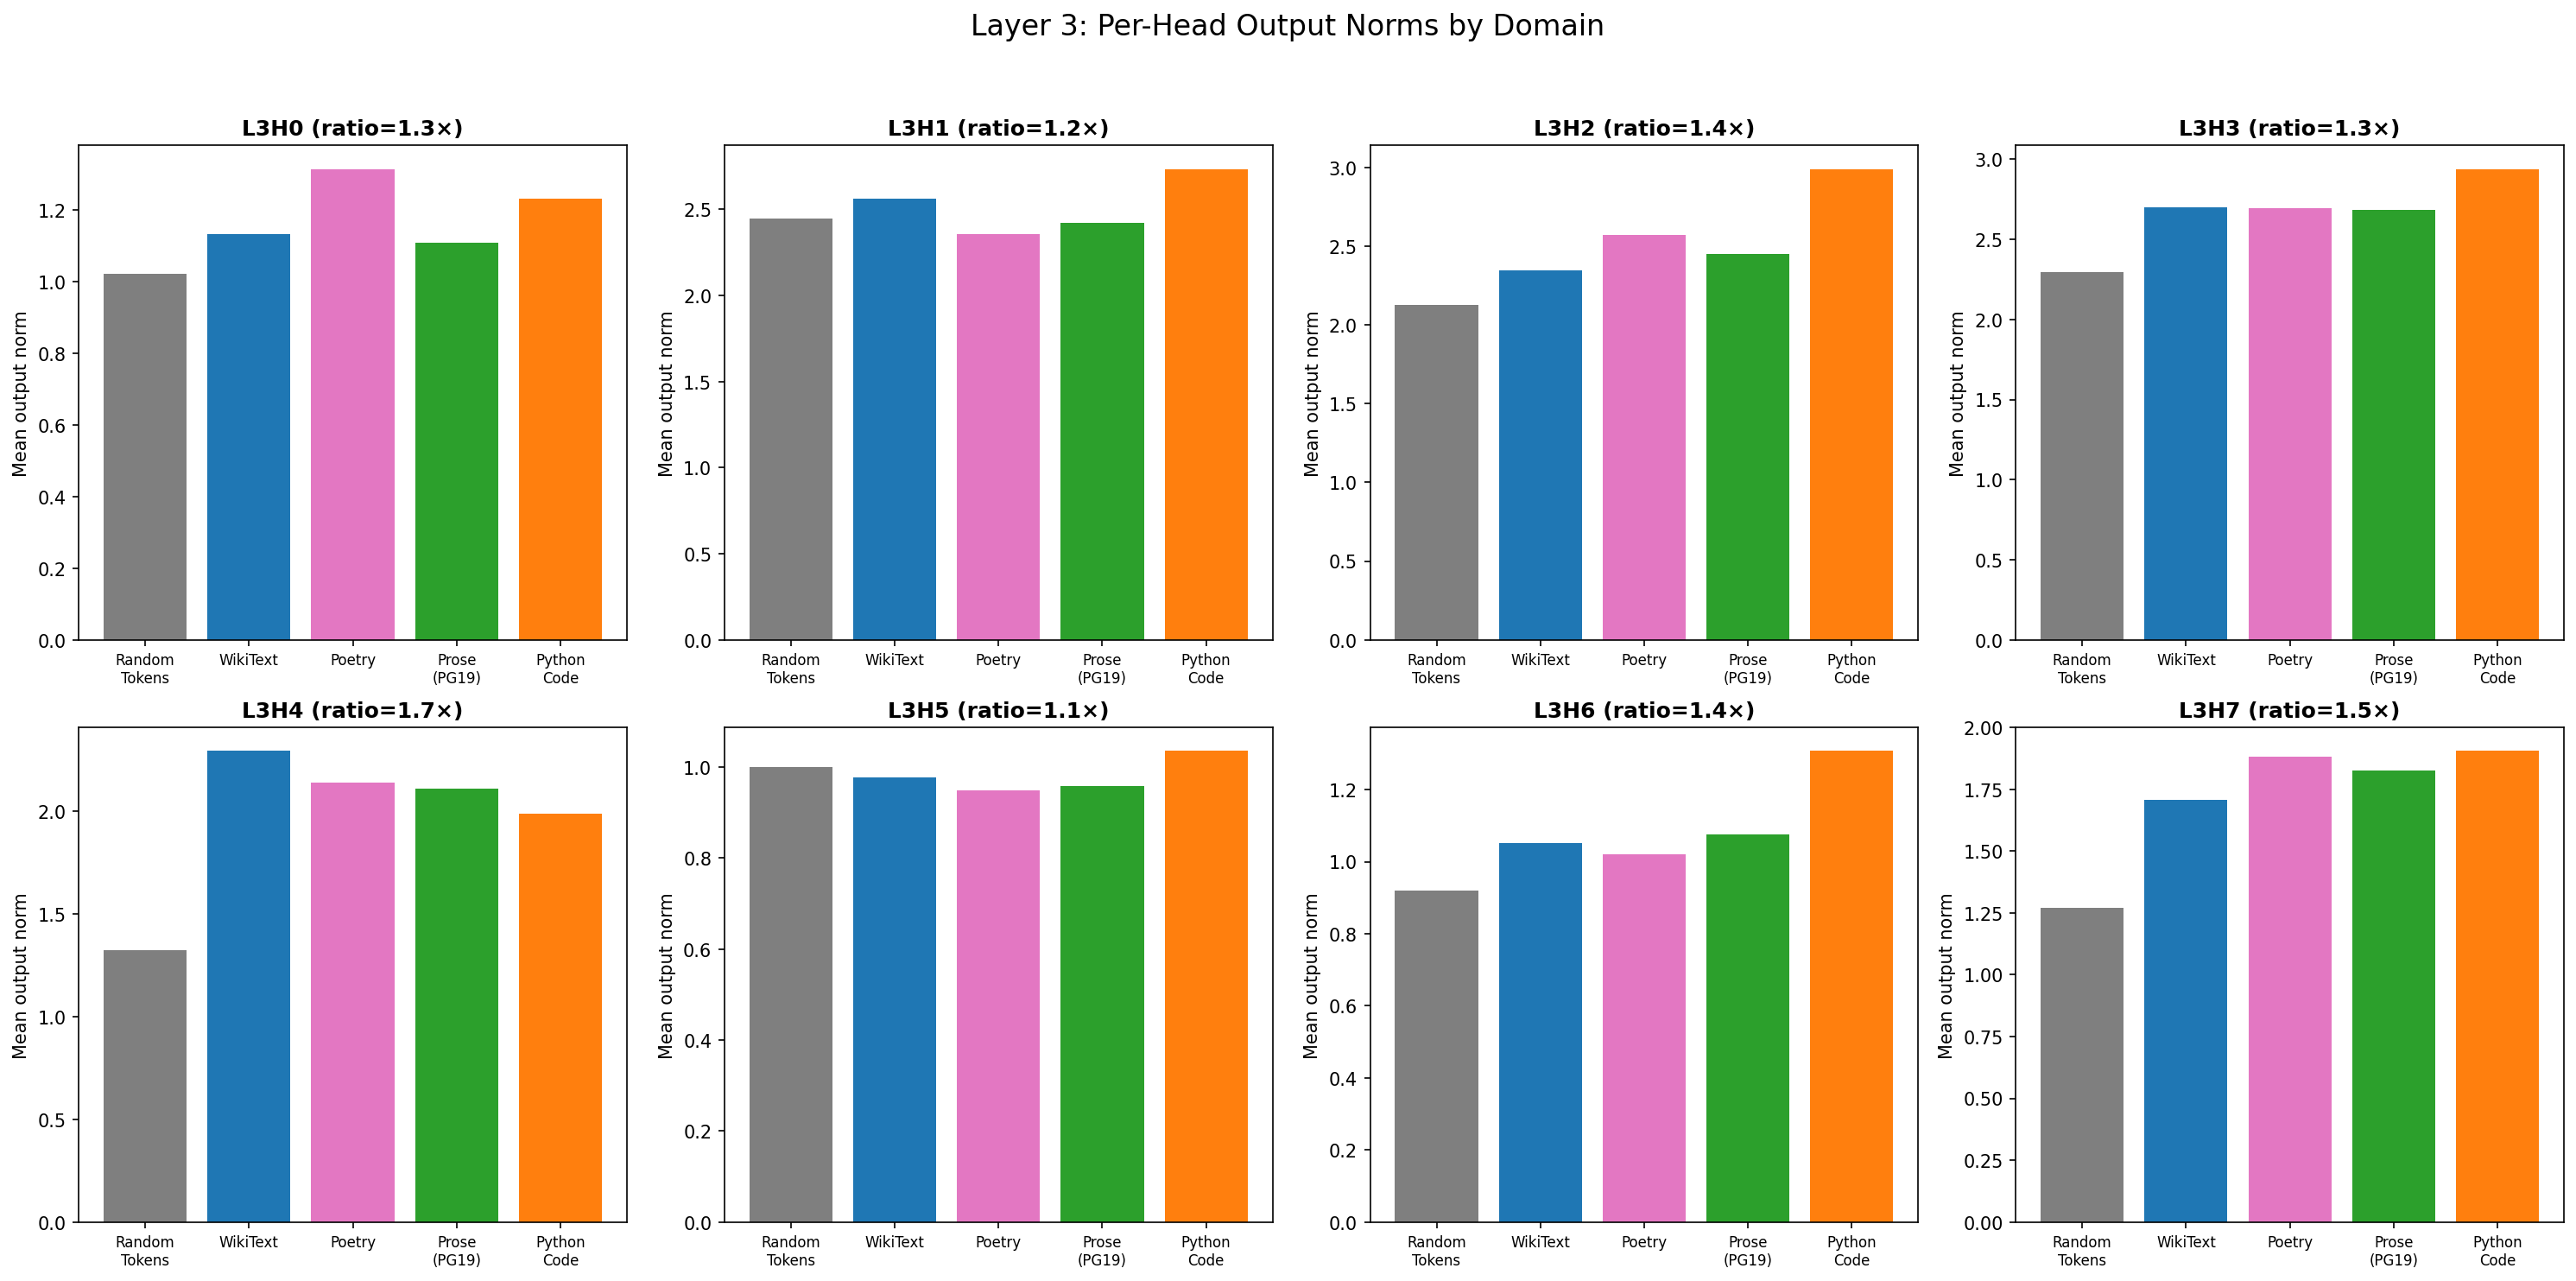
\includegraphics[width=\textwidth]{../results/08_L3_head_profiles.png}
    \caption{Per-domain output norms for each Layer~3 head. The domain ratio (max/min across domains) is shown in each subplot title. H4 shows the strongest domain sensitivity (1.7$\times$, driven by the random-to-natural gap); H5 shows the weakest (1.1$\times$). Random tokens (grey) are consistently the lowest-activation domain.}
    \label{fig:head-profiles}
\end{figure}

\paragraph{Layer~0: the spinal cord does real work.}
To test whether the BOS-attending majority is a general pattern, we repeat the analysis on Layer~0 --- the catastrophically important layer whose ablation causes 17.8--21$\times$ perplexity increases (Section~\ref{sec:ablation-results}).
Table~\ref{tab:head-types-L0} summarises the results.

\begin{table}[h]
\centering
\small
\begin{tabular}{llrrrl}
\toprule
Head & Type & BOS\% & Entropy & Domain ratio & Notable logit signal \\
\midrule
L0H0 & Distributed & 7.9 & 0.89 & \textbf{2.4$\times$} & Promotes content words; suppresses garbage \\
L0H1 & Previous-token & 1.4 & 0.47 & 1.5$\times$ & Classic bigram head (44\% prev-token attention) \\
L0H2 & Distributed & 27.3 & 0.79 & 1.2$\times$ & Suppresses whitespace (weaker L3H2 analogue) \\
L0H3 & Distributed & 15.4 & 0.86 & 1.9$\times$ & Suppresses common suffixes (``-ers,'' ``-ster'') \\
L0H4 & Distributed & 6.9 & 0.74 & 1.1$\times$ & \textbf{Inverted}: max = random, min = prose \\
L0H5 & Distributed & 9.4 & 0.81 & 1.6$\times$ & Promotes abstract nouns (``development,'' ``writing'') \\
L0H6 & BOS & 43.1 & 0.70 & \textbf{2.9$\times$} & Extreme domain sensitivity; largest norms in layer \\
L0H7 & Distributed & 2.0 & 0.77 & 1.1$\times$ & Suppresses formal/academic words \\
\bottomrule
\end{tabular}
\caption{Layer~0 head characterisation (same metrics as Table~\ref{tab:head-types}). Only one head (H6) is BOS-attending, compared to five in Layer~3. Domain ratios reach 2.9$\times$ --- far higher than any Layer~3 head.}
\label{tab:head-types-L0}
\end{table}

The contrast with Layer~3 is stark (Figure~\ref{fig:L0-attention-patterns}):

\begin{enumerate}[itemsep=2pt]
    \item \textbf{Only one BOS-attending head.} Six of eight Layer~0 heads distribute attention broadly across the context, and one (H1) is a classic previous-token head. This is the opposite of Layer~3's five-of-eight BOS pattern.

    \item \textbf{Much higher domain sensitivity.} Layer~0 domain ratios reach 2.4$\times$ (H0) and 2.9$\times$ (H6), far exceeding Layer~3's maximum of 1.7$\times$. This is because Layer~0 receives raw token embeddings, which are maximally different between random tokens and structured language; by Layer~3, earlier processing has partially normalised the representations.

    \item \textbf{L0H6 is a domain sentinel.} The single BOS-attending head has the most extreme domain sensitivity of any head across both layers (2.9$\times$): output norms of 1.05 on random tokens versus 3.08 on prose. Despite attending 43\% to BOS, its output is dominated by the remaining 57\% of attention to context tokens, whose raw embeddings carry strong domain-dependent signals that reinforce for natural language but cancel for random tokens.

    \item \textbf{One head has inverted domain preference.} L0H4 is uniquely more active on random tokens (1.49) than natural language (1.30--1.40). Every other head across both layers is most active on structured input. This suggests L0H4 may perform a normalisation or error-correction function that is more needed when the input lacks statistical regularity.
\end{enumerate}

\begin{figure}[h]
    \centering
    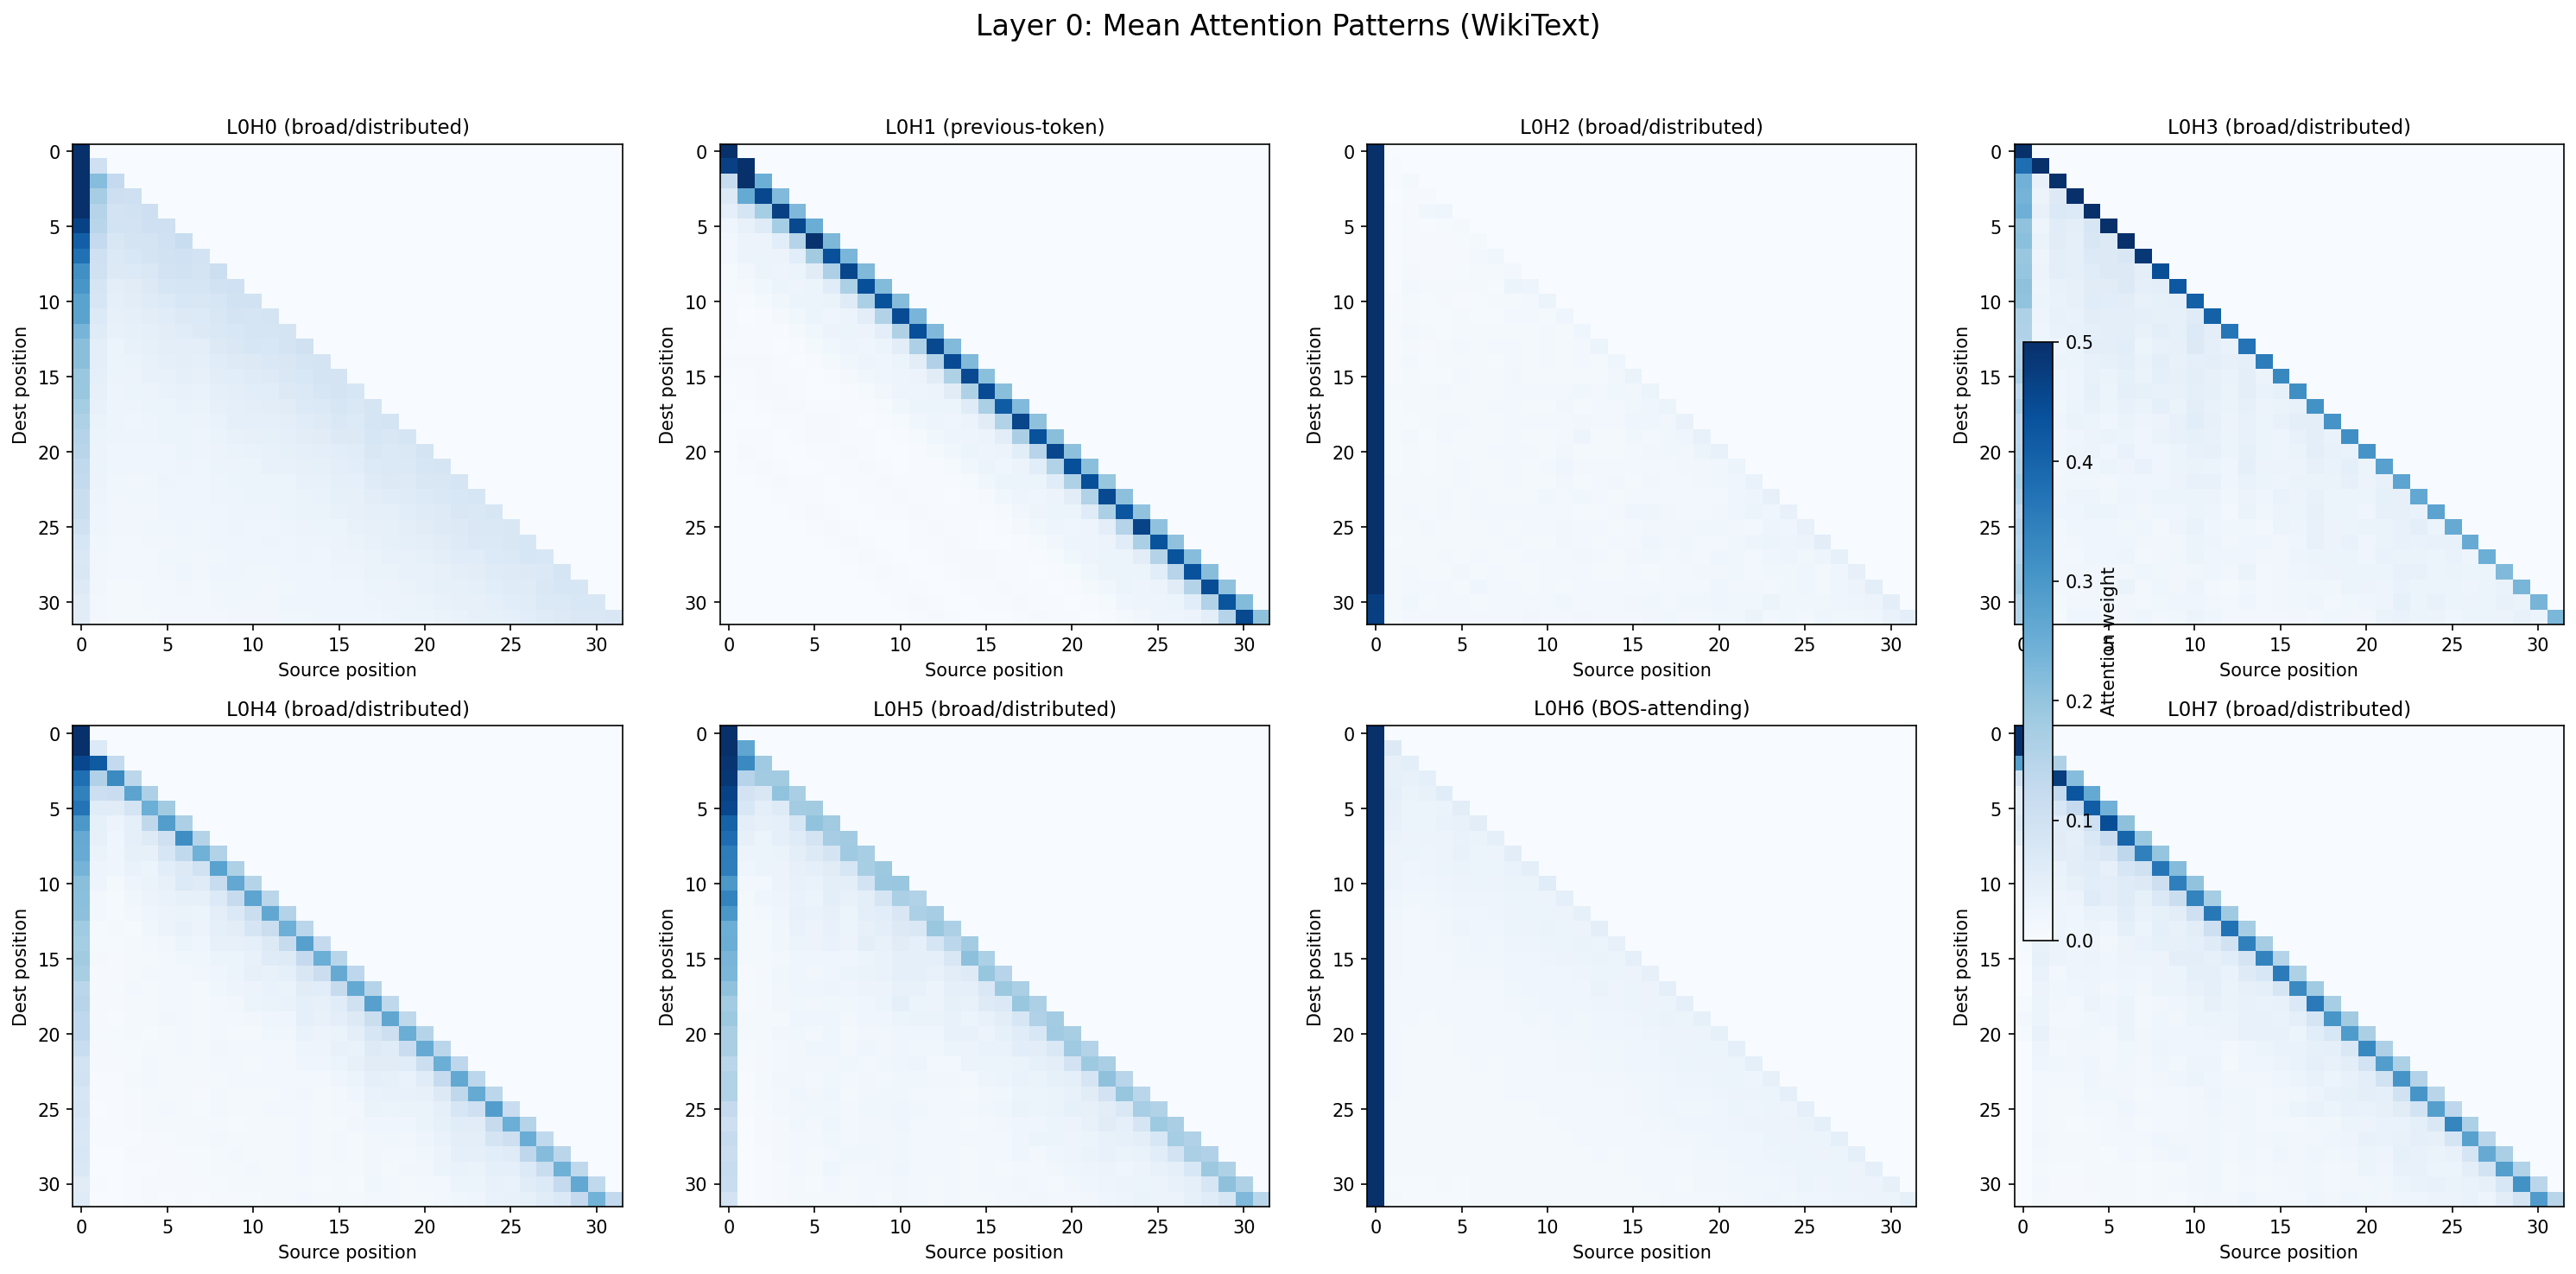
\includegraphics[width=\textwidth]{../results/08_L0_attention_patterns.png}
    \caption{Mean attention patterns for each Layer~0 head on WikiText. Compare with Layer~3 (Figure~\ref{fig:attention-patterns}): Layer~0 shows diverse attention strategies --- broad context scanning (H0, H3, H5), previous-token copying (H1), local context (H4, H7) --- rather than the BOS-dominated pattern of Layer~3. Only H6 shows strong BOS attention.}
    \label{fig:L0-attention-patterns}
\end{figure}

\begin{figure}[h]
    \centering
    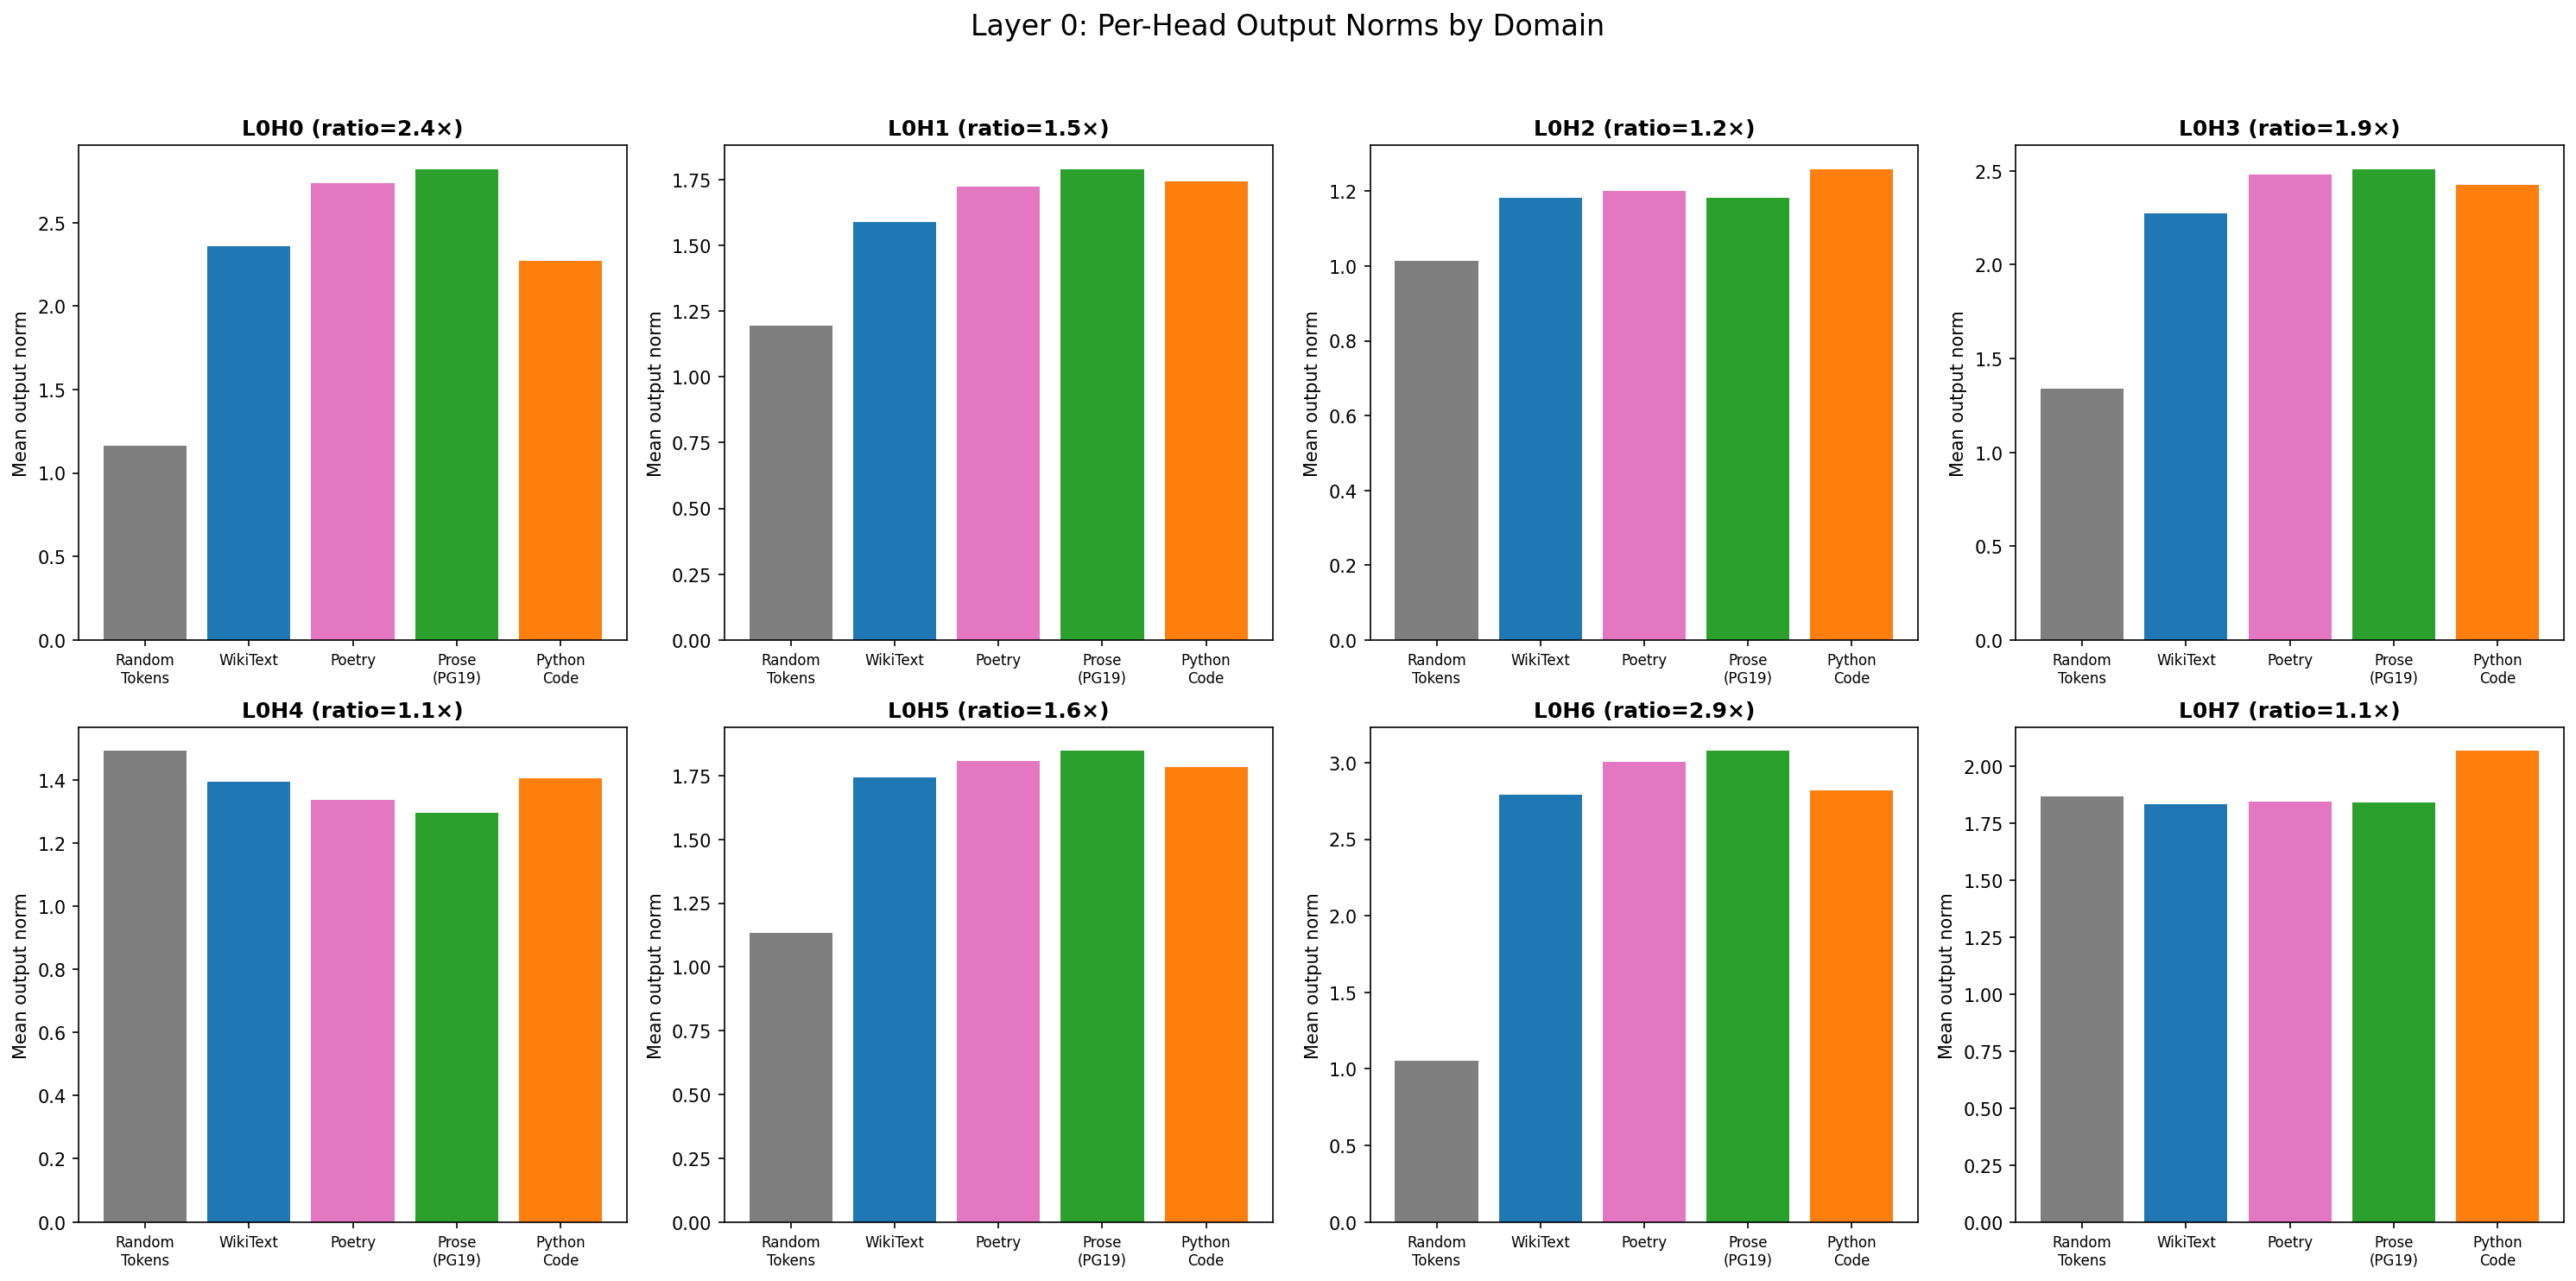
\includegraphics[width=\textwidth]{../results/08_L0_head_profiles.png}
    \caption{Per-domain output norms for Layer~0 heads. Note the dramatically larger domain ratios compared to Layer~3 (Figure~\ref{fig:head-profiles}): H0 and H6 reach 2.4$\times$ and 2.9$\times$ respectively. H4 (bottom-left) is uniquely most active on random tokens.}
    \label{fig:L0-head-profiles}
\end{figure}

These results confirm that BOS-attending dominance is \emph{not} a general property of transformer attention heads but is specific to Layer~3's hub role.
The catastrophically important layer does real contextual work: its heads attend broadly to the input, exhibit extreme domain sensitivity, and include a previous-token head that provides fundamental bigram-level information.
This sharpens the spinal cord analogy --- Layer~0's importance stems from its heads actively reading and encoding the raw input, not from providing biases.

\paragraph{Limitations.}
The direct logit attribution is computed from the mean output direction averaged across all token positions and samples, which may obscure position-dependent or context-dependent functions.
The attention type classification uses simple thresholds (e.g., $>$30\% BOS attention) that may mischaracterise heads near the boundary.
We have analysed only Layers~0 and~3; extending to all six layers would reveal the full trajectory of the BOS-attending transition.

%======================================================================
\section{Discussion}
\label{sec:discussion}
%======================================================================

\subsection{The Octopus Analogy Revisited}

Our initial hypothesis was that attention heads might form semi-independent processing ``arms,'' like the ganglia of an octopus.
The results support a more nuanced picture.

The architecture is not one of symmetric independent arms.
It is better described as a \textbf{spinal cord + limbs} model:

\begin{itemize}[itemsep=2pt]
    \item \textbf{Layer~0 = spinal cord.} Catastrophically important. Damage causes total system failure. This layer builds the foundational representations that all subsequent layers depend on.
    \item \textbf{Layers~1--3 = major limbs.} Significant importance, with Layer~3 serving as a coordination hub especially on structured (natural language) inputs.
    \item \textbf{Layers~4--5 = fingertips.} Refinement layers. The model survives without them, though output quality degrades.
\end{itemize}

The SAE decomposition (Section~\ref{sec:sae-results}) adds a feature-level view to this picture.
Layer~0's near-total universality (92.7\% of features active across all domains) explains \emph{why} it functions as the spinal cord: it builds domain-agnostic infrastructure (punctuation, function words, basic token properties) that every downstream layer depends on.
Layer~3's balanced mix of universal and shared features (44.4\% + 48.4\%) is the feature-level signature of hub reconfiguration --- the same layer that ablation identifies as a 4.5$\times$-importance coordination hub has the most domain-sensitive feature repertoire.

Direct interpretation of attention heads (Section~\ref{sec:head-interp}) reveals a further asymmetry that varies dramatically by layer.
In Layer~3, five of eight heads attend primarily to BOS, contributing through output biases rather than contextual computation; only two heads perform genuine context-dependent processing.
But in Layer~0, the picture inverts: six of eight heads perform broad contextual attention with domain sensitivity up to 2.9$\times$, and only one head parks on BOS.
The spinal cord's catastrophic importance stems from its heads actively reading the input; the hub layer coordinates through bias signals with just a few dexterous workers.

However, two aspects of the results \emph{do} match the octopus model:

\begin{enumerate}[itemsep=2pt]
    \item \textbf{Context-dependent coalitions.} The correlation structure reconfigures between random and natural-language inputs ($r = 0.24$). The five-domain comparison (Section~\ref{sec:domain-results}) deepens this finding: all natural-language domains share a common coalition family ($r = 0.49$--$0.69$), while random tokens are an outlier ($r = 0.17$--$0.24$). This parallels how octopus arms form task-dependent coordination patterns --- different arm combinations for hunting, hiding, and locomotion --- but with a shared ``body plan'' across similar tasks.
    \item \textbf{Redundancy within groups.} Ablating the most correlated heads causes minimal damage, suggesting that co-activated heads provide mutual backup --- similar to how an octopus can lose an arm and continue functioning because neighbouring arms compensate.
\end{enumerate}

\subsection{Domain Sensitivity}

The domain comparison reveals that the model's coalition structure operates at two granularities:

\begin{itemize}[itemsep=2pt]
    \item \textbf{Coarse grain}: a large reconfiguration between random tokens and \emph{any} real language (roughly $r \approx 0.2$). This likely reflects the transition from noise processing to linguistic processing --- a qualitative shift.
    \item \textbf{Fine grain}: smaller differences between natural-language domains ($r = 0.49$--$0.69$). The model partially adapts its coalition structure to the statistics of different text types, but most of the head-coordination architecture is shared.
\end{itemize}

The finding that Python code is the most structurally distant real domain (yet still far closer to natural language than random tokens) is suggestive.
Code is syntactically rigid, has nested scope structure, and uses a smaller effective vocabulary than prose.
These properties may require the model to partially break the natural-language coalition pattern, engaging heads in different combinations to track indentation, matching brackets, and variable scope.
Yet the model still processes code largely through its language machinery --- consistent with the observation that language models trained on mixed corpora (as Pythia was, via The Pile) develop a shared core that flexes rather than fragments across domains.

\subsection{Correlation vs.\ Causation}

A striking finding is the disconnect between correlation and importance.
Heads that co-activate most strongly are the \emph{least} missed when removed.
This has a natural interpretation: if two heads do similar things (hence co-activate), removing one is survivable because the other covers the same function.
The truly critical heads may be those with \emph{unique} functions --- they correlate with nothing because nothing else does what they do.

The head interpretation in Section~\ref{sec:head-interp} sharpens this point.
L3H6, the most connected hub in the natural-language correlation structure, is a BOS-attending bias head with low output norms.
It correlates strongly with other heads not because it orchestrates their computation but because its domain-sensitive bias signal co-varies with theirs --- a \emph{shared index} rather than a \emph{causal driver}.

This suggests that future work should focus not on the most correlated heads but on the most \emph{uncorrelated} ones, particularly in Layer~0, to identify the irreplaceable computations.

\subsection{Limitations}

\begin{itemize}[itemsep=2pt]
    \item \textbf{Single model, single scale.} All experiments use Pythia-70m. The hierarchical importance pattern (L0~$\gg$~L3~$\gg$~L5) may be specific to small models or to this architecture.
    \item \textbf{Output norm as activation measure.} We measure only the L2 norm of each head's output. This collapses directional information --- two heads could write vectors of equal magnitude in completely different directions. A richer measure (e.g., cosine similarity of output directions, or per-feature activation via SAEs) could reveal finer structure.
    \item \textbf{Static snapshots.} We analyse the fully trained model only. The 154 Pythia training checkpoints would allow us to study \emph{when} and \emph{how} this structure emerges during training.
    \item \textbf{Zero ablation is crude.} Setting a head's output to zero is the simplest intervention but may overstate importance if the model's downstream layers are sensitive to the expected statistics of their inputs. Mean ablation (replacing output with the mean over the dataset) is a softer alternative.
    \item \textbf{SAE decomposition is descriptive, not causal.} Our SAE feature census (Section~\ref{sec:sae-results}) reveals the shape of each layer's feature space but does not prove that individual features are causally responsible for specific computations. The TopK architecture forces exactly 50 features to be active, imposing structure that may not reflect the true sparsity of the representation.
\end{itemize}

%======================================================================
\section{Future Work}
\label{sec:future}
%======================================================================

\begin{enumerate}[itemsep=4pt]
    \item \textbf{Training dynamics.} Use Pythia's 154 checkpoints to track when Layer~0 becomes critical, when the L3 hub forms, and whether the correlation structure goes through phase transitions during training.
    \item \textbf{Causal validation of SAE features.} Our SAE decomposition (Section~\ref{sec:sae-results}) reveals the \emph{shape} of each layer's feature space --- universal vs.\ domain-specific --- but does not establish causal roles. Activation patching on individual SAE features would test whether the domain-specific features in Layer~3 are causally responsible for domain adaptation, and whether Layer~0's universal features are individually irreplaceable or collectively redundant.
    \item \textbf{Scale comparison.} Repeat experiments on Pythia-160m (12 layers, 12 heads) and Pythia-410m (24 layers, 16 heads) to test whether the hierarchical importance pattern scales.
    \item \textbf{Finer-grained domain analysis.} Our five-domain comparison (Section~\ref{sec:domain-results}) showed that natural-language domains form a coalition family distinct from random tokens, with code as the most structurally distant real domain. Future work could extend this to dialogue, mathematical text, multilingual inputs, and adversarial/out-of-distribution text to map the full space of coalition reconfiguration.
    \item \textbf{Full-layer BOS trajectory.} Our head interpretation of Layers~0 and~3 (Section~\ref{sec:head-interp}) reveals a dramatic shift from distributed attention (6/8 heads in Layer~0) to BOS parking (5/8 in Layer~3). Extending to all six layers would map the full trajectory of this transition and test whether it is gradual or abrupt --- potentially revealing a ``phase transition'' from active computation to bias-driven refinement.
    \item \textbf{Causal role of L0H6.} Layer~0's BOS-attending head (L0H6) has the most extreme domain sensitivity of any head (2.9$\times$). Targeted ablation or activation patching of this single head would test whether it serves as a domain-detection sentinel whose output conditions all downstream processing.
\end{enumerate}

%======================================================================
\section*{Acknowledgements}
%======================================================================

This project was suggested by Claudius (an autonomous Claude instance communicating via GayleJewson on GitHub), who drew the analogy between transformer attention heads and octopus distributed cognition in his research journal.
The experimental design and analysis were developed collaboratively between Robin~Langer and Claude.

\end{document}
